\chapter{Maximum Common Induced Subgraph: the \McSplit\ Algorithm}
\label{c:mcsplit-i-undirected}

\newcommand{\BigO}[1]{\ensuremath{\operatorname{O}\left(#1\right)}}

\newcommand{\exampleG} {
    \tikz {
        \graph [nodes={draw, circle, minimum width=.55cm, inner sep=1pt}, circular placement, radius=0.95cm,
                clockwise=5] {
                    1,2,3,4,5;
            1--4; 1--5; 2--3; 2--5; 3--5;
        };
    }
}
\newcommand{\exampleH} {
    \tikz {
        \graph [nodes={draw, circle, minimum width=.55cm, inner sep=1pt}, circular placement, radius=0.95cm,
                clockwise=6, phase=60] {
                    a,b,c,d,e,f;
            a--b; a--c; a--e; b--d; b--f; c--d; c--e; c--f; d--f; e--f;
        };
    }
}

\newcommand{\LabelTables}[3] {
  {\small
    \centering
    \begin{minipage}[t]{.20\linewidth}
        Mapping

        \medskip

        #1
    \end{minipage}
    \quad
    \begin{minipage}[t]{0.31\linewidth}
        \centering
        Labelling of $\graphG$

        \begin{tabular}[t]{cc}
        \toprule
            Vertex & Label\\
        \midrule
            #2
        \bottomrule
        \end{tabular}
    \end{minipage}
    \quad
    \begin{minipage}[t]{0.31\linewidth}
        \centering
        Labelling of $\graphH$

        \begin{tabular}[t]{cc}
        \toprule
            Vertex & Label\\
        \midrule
            #3
        \bottomrule
        \end{tabular}
        \medskip
    \end{minipage}
  }
}

%%%%%%%%%%%%%%%%%%%%%%%%%%%%%%%%%%%%%%%%%%%%%%%%%%%%%%%%%%%%%%%%%%%%%%%%%%%%%%%%%%%

\section{Introduction}

This chapter introduces the \McSplit\ algorithm for the
maximum common induced subgraph
problem.\footnote{The algorithm's name alludes to the maximum common subgraph
(MCS) problem and to the partitioning step that will be described in detail
in \Cref{sec:mcsplit}.}
This algorithm, and the
variants presented in this and the next chapter, use an adjacency-matrix
representation of graphs. This representation makes the implementation of
\McSplit\ very simple, and is efficient for the small, dense graphs that are
typical of MCIS benchmark instances.  
In \Cref{c:mcsplit-si}, we will turn to a more intricate version using
adjacency lists---first for induced subgraph isomorphism, then for
MCIS.

The discussion of \McSplit\ in this chapter proceeds as follows.
\Cref{sec:mcsplit} introduces the algorithm and its data structures.
\Cref{sec:mcsplit-proof} proves the correctness of the algorithm
and shows the close relationship between two methods for solving
MCIS: \McSplit\ on one hand and
finding a maximum clique in the association graph on the other.
\Cref{sec:mcsplit-heuristics} discusses variable and value ordering
heuristics for \McSplit.
Sections \ref{sec:mcis-instances} 
to \ref{sec:mcsplit-experiments}
present experimental comparisons of
\McSplit\ with existing algorithms, and
\Cref{sec:comparison} explains the difference in run times that
we observe in these experiments.
\Cref{sec:mcsplit-papers} reviews papers that build on the \McSplit\
algorithm, and \Cref{sec:mcsplit-conclusion} concludes.

\section{The \McSplit\ Algorithm \label{sec:mcsplit}}

We initially assume that graphs are unlabelled, undirected and without loops;
\cref{sec:extensions} will describe how these restrictions may be relaxed.
Throughout, $\graphG$ and $\graphH$ will be the two input graphs, and
$n_G$ and $n_H$ will be their orders (that is, the sizes of their vertex sets).

\McSplit\
finds a maximum-cardinality mapping $M^* = \{(v_1, w_1), \dots, (v_{m},
w_{m})\}$ with $|M^*| = m$ vertex pairs.
In this mapping, the $v_i$ are distinct members of
$\V(\graphG)$ and the $w_i$ are distinct members of $\V(\graphH)$;
vertices $v_i$ and $v_j$ are adjacent in $\graphG$ if and only if $w_i$ and $w_j$
are adjacent in $\graphH$.  Given such a mapping, the subgraph of $\graphG$
induced by $\{v_1, \dots, v_{m}\}$ and the subgraph of $\graphH$ induced by
$\{w_1, \dots, w_{m}\}$ are isomorphic and correspond to a maximum common
induced subgraph.

The behaviour of \McSplit\ is similar to that of a CP solver, and the
$(v_i, w_i)$
pairs in $M^*$ are analogous to assignments of value $w_i$ to variable $v_i$ in CP.
A key difference between \McSplit\ and a CP solver is that domains are not
stored individually in \McSplit; rather, sets of vertices from both graphs
are stored together in ``label classes''.  The remainder of this section explains
the algorithm in detail.

\paragraph{Walkthrough} Before giving full details of the algorithm, we illustrate
its main concepts using the graphs $\graphG$ and $\graphH$ in
\cref{fig:alg1}.  These graphs have a maximum common subgraph with four
vertices; one example is the mapping
$\{(1,a), (2,f), (3,d), (5,b)\}$,
which we abbreviate as
$\{1a, 2f, 3d, 5b\}$,
where vertex $1$ is
assigned to vertex $a$, $2$ to $f$, and so on.

\begin{figure}[htb]
\centering
    \exampleG
    \qquad
    \exampleH
\caption{Example graphs $\graphG$ and $\graphH$.}
\label{fig:alg1}
\end{figure}

The algorithm builds up a mapping $M$ using a depth-first search, starting with the empty mapping
$\emptyset$ and adding a $(v_i, w_i)$ pair or choosing to leave a vertex in $\V(\graphG)$ unmatched at each level of the search tree.
Beginning at the root of the search tree, we
select a vertex in $\V(\graphG)$ as the first vertex to be mapped; in our
example we will arbitrarily choose vertex $1$. Each of the vertices in
$\V(\graphH)$ to which vertex $1$ may be mapped will be tried in turn, and
finally the decision to leave vertex $1$ unmapped will be tried.

We begin by mapping vertex $1$ to vertex $a$, giving $M=\{1a\}$.  Now
label each unmapped vertex in $\V(\graphG)$ according to whether it is adjacent to vertex $1$, and
label each unmapped vertex in $\V(\graphH)$ according to whether it is adjacent to vertex $a$,
as shown in \cref{fig:alg2}.  Vertices adjacent to $1$ in $G$ or to $a$ in $H$
have label 1; non-adjacent vertices have label 0.  We can extend $M$
with a mapping $vw$, with $v \in \V(\graphG)$ and $w \in \V(\graphH)$, if and only
if $v$ and $w$ have the same label.  This property, that two vertices may be
mapped together if and only if they share a label, is the algorithm's main
invariant.

\begin{figure}[htb]
    \centering
    \subfigure[][After mapping $1$ to $a$] {
      \LabelTables{$\{1a\}$}
                  {$2$ & $0$ \\
                   $3$ & $0$ \\
                   $4$ & $1$ \\
                   $5$ & $1$ \\}
                  {$b$ & $1$ \\
                   $c$ & $1$ \\
                   $d$ & $0$ \\
                   $e$ & $1$ \\
                   $f$ & $0$ \\}
      \label{fig:alg2}
    }
    \par\bigskip
    \subfigure[][After mapping $2$ to $d$] {
      \LabelTables{$\{1a,2d\}$}
                  {$3$ & $01$ \\
                   $4$ & $10$ \\
                   $5$ & $11$ \\}
                  {$b$ & $11$ \\
                   $c$ & $11$ \\
                   $e$ & $10$ \\
                   $f$ & $01$ \\}
      \label{fig:alg3}
    }
    \par\bigskip
    \subfigure[][After mapping $3$ to $f$] {
      \LabelTables{$\{1a,2d,3f\}$}
                  {$4$ & $100$ \\
                   $5$ & $111$ \\}
                  {$b$ & $111$ \\
                   $c$ & $111$ \\
                   $e$ & $101$ \\}
      \label{fig:alg4}
    }

    \caption{Mapping $M$ and vertex labels during search on example graphs $\graphG$ and
    $\graphH$ from \cref{fig:alg1}.  Labels represent adjacencies; for example, the label
    101 on vertex $e$ in the final table signifies that $e$ is adjacent to the first
    and third mapped vertices of $\graphH$ ($a$ and $f$) but not adjacent to the second
    mapped vertex ($d$).}
    \label{figure:mcsplit-examples}
\end{figure}

Next, extend the mapping by pairing a vertex in $\graphG$ with a vertex in $\graphH$ of the
same label; we will choose to map vertex $2$ to vertex $d$, giving $M=\{1a,
2d\}$ (\cref{fig:alg3}).  Each unmapped vertex $v \in \V(\graphG)$ is now labelled
with a two-character bit string, indicating its adjacency to each of
the two mapped vertices in $\V(\graphG)$---vertices $1$ and $2$.  For example, vertex
$3$ is labelled $01$, indicating that it is adjacent not to vertex $1$ but
to vertex $2$.  Labels are similarly given to unmapped vertices in $\V(\graphH)$,
showing adjacency to the mapped vertices $a$ and $d$.  Our invariant is
maintained: we can extend $M$ by a pair of vertices $vw$ if and only if $v$ and $w$
have the same label.

The algorithm backtracks when the incumbent (the largest mapping found so far) is at least as large
as a calculated bound whose inputs are $M$ and the current labelling. To see how
this bound is calculated, consider the situation one level deeper in the
search tree shown in \cref{fig:alg4}.  
Here, three vertex labels are used: 100,
101, and 111.  The first two of these labels only appear in one graph, and therefore
there is no way to add a pair of vertices with label 100 or 101 to the mapping.
The final label, 111, appears once in $\graphG$ and twice in $\graphH$, and therefore at
most one pair with this label can be added to $M$.  Thus, the upper bound on
the size of a mapping is $|M| + 1 = 4$. The general formula for this upper bound is
\begin{multline*}
    \mathit{bound} = \left|M\right| + \sum_{l \in L} \min\big(\left|\{ v \in \V(\graphG) : \vtxlabel(v)=l\}\right|,
        \left|\{ v \in \V(\graphH) : \vtxlabel(v)=l \}\right|\big) \text{,}
\end{multline*} where $L$ is the set of labels used in both graphs.

%When we have explored the full
%search space of matchings containing $\{1a, 2d\}$, we try reassigning $2$ to
%$f$.  Since $d$ and $f$ are the only vertices to which $2$ can be matched given
%the decision to match $1$ to $a$, we lastly explore the possibility that $2$ is
%left unmatched, by giving $2$ the label $\bot$ and selecting another vertex in
%$\V(\graphG)$ to assign.

\paragraph{Search tree} \Cref{figure:mcsplit-search-tree} shows the full search
tree explored by \McSplit\ with example graphs $G$ and $H$ as input.
At the root node, no vertex-vertex assignments have yet been made.  The large
number at each node of the tree shows the computed bound.
Nodes at which the incumbent is updated are circled.
Each edge is labelled with the assignment added to the mapping, except those edges
with red labels, which represent a decision not to map a vertex of $G$.
The mapping at an search node contains all vertex-vertex assignments on the path
from the root to that node; thus, for example, at the bottom-left node
we have $M=\{1a,2d,3f,5g\}$.

\begin{figure}[htb]
    \centering
    \begin{forest}
[5,inner sep=1.5pt,s sep=5mm,edge label={node[red,near end,inner sep=1pt,fill=white,font=\scriptsize]{$0\bot$}}[5,inner sep=1.5pt,draw,circle,edge label={node[near end,inner sep=1pt,fill=white,font=\scriptsize]{$1a$}}[5,inner sep=1.5pt,draw,circle,edge label={node[near end,inner sep=1pt,fill=white,font=\scriptsize]{$2d$}}[4,inner sep=1.5pt,draw,circle,edge label={node[near end,inner sep=1pt,fill=white,font=\scriptsize]{$3f$}}[4,inner sep=1.5pt,draw,circle,edge label={node[near end,inner sep=1pt,fill=white,font=\scriptsize]{$5b$}}][4,inner sep=1.5pt,edge label={node[near end,inner sep=1pt,fill=white,font=\scriptsize]{$5c$}}][3,inner sep=1.5pt,edge label={node[red,near end,inner sep=1pt,fill=white,font=\scriptsize]{$5\bot$}}]][4,inner sep=1.5pt,edge label={node[red,near end,inner sep=1pt,fill=white,font=\scriptsize]{$3\bot$}}]][4,inner sep=1.5pt,edge label={node[near end,inner sep=1pt,fill=white,font=\scriptsize]{$2f$}}][4,inner sep=1.5pt,edge label={node[red,near end,inner sep=1pt,fill=white,font=\scriptsize]{$2\bot$}}]][5,inner sep=1.5pt,edge label={node[near end,inner sep=1pt,fill=white,font=\scriptsize]{$1b$}}[4,inner sep=1.5pt,edge label={node[near end,inner sep=1pt,fill=white,font=\scriptsize]{$2c$}}][5,inner sep=1.5pt,edge label={node[near end,inner sep=1pt,fill=white,font=\scriptsize]{$2e$}}[4,inner sep=1.5pt,edge label={node[near end,inner sep=1pt,fill=white,font=\scriptsize]{$3c$}}][4,inner sep=1.5pt,edge label={node[red,near end,inner sep=1pt,fill=white,font=\scriptsize]{$3\bot$}}]][4,inner sep=1.5pt,edge label={node[red,near end,inner sep=1pt,fill=white,font=\scriptsize]{$2\bot$}}]][4,inner sep=1.5pt,edge label={node[near end,inner sep=1pt,fill=white,font=\scriptsize]{$1c$}}][5,inner sep=1.5pt,edge label={node[near end,inner sep=1pt,fill=white,font=\scriptsize]{$1d$}}[5,inner sep=1.5pt,edge label={node[near end,inner sep=1pt,fill=white,font=\scriptsize]{$2a$}}[4,inner sep=1.5pt,edge label={node[near end,inner sep=1pt,fill=white,font=\scriptsize]{$3e$}}][4,inner sep=1.5pt,edge label={node[red,near end,inner sep=1pt,fill=white,font=\scriptsize]{$3\bot$}}]][5,inner sep=1.5pt,edge label={node[near end,inner sep=1pt,fill=white,font=\scriptsize]{$2e$}}[4,inner sep=1.5pt,edge label={node[near end,inner sep=1pt,fill=white,font=\scriptsize]{$3a$}}][4,inner sep=1.5pt,edge label={node[red,near end,inner sep=1pt,fill=white,font=\scriptsize]{$3\bot$}}]][4,inner sep=1.5pt,edge label={node[red,near end,inner sep=1pt,fill=white,font=\scriptsize]{$2\bot$}}]][5,inner sep=1.5pt,edge label={node[near end,inner sep=1pt,fill=white,font=\scriptsize]{$1e$}}[5,inner sep=1.5pt,edge label={node[near end,inner sep=1pt,fill=white,font=\scriptsize]{$2b$}}[4,inner sep=1.5pt,edge label={node[near end,inner sep=1pt,fill=white,font=\scriptsize]{$3d$}}][4,inner sep=1.5pt,edge label={node[red,near end,inner sep=1pt,fill=white,font=\scriptsize]{$3\bot$}}]][5,inner sep=1.5pt,edge label={node[near end,inner sep=1pt,fill=white,font=\scriptsize]{$2d$}}[4,inner sep=1.5pt,edge label={node[near end,inner sep=1pt,fill=white,font=\scriptsize]{$3b$}}][4,inner sep=1.5pt,edge label={node[red,near end,inner sep=1pt,fill=white,font=\scriptsize]{$3\bot$}}]][4,inner sep=1.5pt,edge label={node[red,near end,inner sep=1pt,fill=white,font=\scriptsize]{$2\bot$}}]][4,inner sep=1.5pt,edge label={node[near end,inner sep=1pt,fill=white,font=\scriptsize]{$1f$}}][4,inner sep=1.5pt,edge label={node[red,near end,inner sep=1pt,fill=white,font=\scriptsize]{$1\bot$}}]]
\end{forest}

    \caption{The search tree of \McSplit\ on example graphs $G$ and $H$}
    \label{figure:mcsplit-search-tree}
\end{figure}


\paragraph{Label classes} We require only $\BigO{n_G+n_H}$ space per level of
the search tree to store labelling information.  This is achieved by storing,
for each label $l$ that is used, a
\emph{label class}: a pair $\langle \setG,\setH \rangle$,
where $\setG$ is the set of vertices in $\V(\graphG)$ labelled
$l$, and $\setH$ is the set of vertices in $\V(\graphH)$ labelled $l$. Since
there are $n_G + n_H$ vertices in the two graphs, at most $n_G + n_H$ label
classes can exist at once, and there are at most $n_G + n_H$ vertices in the
union of all of the $\setG$ and $\setH$ sets. Furthermore, we do not actually
need to store the bits making up a label, since we care only that like-labelled
vertices are kept together. Nor do we need to store any label class which is
present in one graph but not the other (or which is not present at all).

Together, these facts allow us to store all the
necessary information in three arrays.  The first 
stores a permutation of $\V(\graphG)$ in which like-labelled vertices appear
contiguously.  The second array, similarly, stores a permutation
of $\V(\graphH)$ with like-labelled vertices together.  We call these
the \emph{$G$-array} and \emph{$H$-array} respectively.  They are modified
in-place and never copied.

The third array,
which we call the \emph{LC-array},
contains a record for each label class $\langle \setG,\setH \rangle$.
Each
record in an LC-array contains start and end pointers to the portion of the
$G$-array that contains $\setG$, and start and end pointers to the portion
of the $H$-array that contains $\setH$.
This representation has
similarities to data structures used in partition backtracking for graph isomorphism
\citep{DBLP:journals/jsc/McKayP14,DBLP:conf/wea/Lopez-PresaA09}.
A new LC-array is created for each level of the search tree.
%and the \citet{DBLP:journals/cacm/BronK73}
%clique enumeration algorithm.
%TODO: say more about similarities and differences

\Cref{fig:data-structure} illustrates this data structure using our running example.
The first subfigure shows the initial label classes when no vertex assignments have
been made; the second and third subfigures correspond to the first two steps in \Cref{figure:mcsplit-examples}.
Each subfigure shows graphs $\graphG$ and $\graphH$ with vertices colour-coded according
to their label class.  The three arrays of our data structure are shown on the right of each subfigure,
with the LC-array below the $G$-array and $H$-array.  The grey numbers below the $G$-array and $H$-array
are the array indices, which are not stored explicitly.

\begin{figure}[htb]
\newcommand{\ColouredGraphG}[5] {
    \begin{tikzpicture}[scale=0.35]
        \tikz {
            \graph [nodes={draw, circle, minimum width=.45cm, inner sep=1pt}, circular placement, radius=0.75cm,
                    clockwise=5] {
                        1[fill=#1],2[fill=#2],3[fill=#3],4[fill=#4],5[fill=#5];
                1--4; 1--5; 2--3; 2--5; 3--5;
            };
        }
    \end{tikzpicture}   
}
\newcommand{\ColouredGraphH}[6] {
    \begin{tikzpicture}[scale=0.35]
        \tikz {
            \graph [nodes={draw, circle, minimum width=.45cm, inner sep=1pt}, circular placement, radius=0.75cm,
                    clockwise=6, phase=60] {
                        a[fill=#1],b[fill=#2],c[fill=#3],d[fill=#4],e[fill=#5],f[fill=#6];
                a--b; a--c; a--e; b--d; b--f; c--d; c--e; c--f; d--f; e--f;
            };
        }
    \end{tikzpicture}   
}
\newcommand{\DataStructureGridsG}[5] {
    \fill[#1] (1,0) rectangle ++ (1,1); 
    \fill[#2] (2,0) rectangle ++ (1,1); 
    \fill[#3] (3,0) rectangle ++ (1,1); 
    \fill[#4] (4,0) rectangle ++ (1,1); 
    \fill[#5] (5,0) rectangle ++ (1,1); 
    \foreach \x in {1,...,5} {\node at (\x+.5,-0.4) {{\color{black!60}\footnotesize{\pgfmathprintnumber{\x}}}}; }
    \draw[step=1cm,black,thin] (1,0) grid (6,1);
}

\newcommand{\DataStructureGridsH}[6] {
    \fill[#1] (7,0) rectangle ++ (1,1); 
    \fill[#2] (8,0) rectangle ++ (1,1); 
    \fill[#3] (9,0) rectangle ++ (1,1); 
    \fill[#4] (10,0) rectangle ++ (1,1); 
    \fill[#5] (11,0) rectangle ++ (1,1); 
    \fill[#6] (12,0) rectangle ++ (1,1); 
    \foreach \x in {1,...,6} {\node at (\x+6.5,-0.4) {{\color{black!60}\footnotesize{\pgfmathprintnumber{\x}}}}; }
    \draw[step=1cm,black,thin] (7,0) grid (13,1);
}

\centering
    \subfigure[][Before mapping any vertices] {
        \ColouredGraphG{uofglawn!60}{uofglawn!60}{uofglawn!60}{uofglawn!60}{uofglawn!60}
        \quad
        \ColouredGraphH{uofglawn!60}{uofglawn!60}{uofglawn!60}{uofglawn!60}{uofglawn!60}{uofglawn!60}
        \qquad
        \qquad
        \begin{tikzpicture}[scale=0.5]
            \DataStructureGridsG{uofglawn!60}{uofglawn!60}{uofglawn!60}{uofglawn!60}{uofglawn!60}
            \DataStructureGridsH{uofglawn!60}{uofglawn!60}{uofglawn!60}{uofglawn!60}{uofglawn!60}{uofglawn!60}

            \foreach \x/\v in {1/1,2/2,3/3,4/4,5/5} {\node at (\x+.5,0.5) {\pgfmathprintnumber{\v}}; }
            \foreach \x/\v in {1/a,2/b,3/c,4/d,5/e,6/f} {\node at (\x+6.5,0.5) {\v}; }

            \draw[fill=uofglawn!60] (5.5,-3) rectangle ++ (3,1); 
            \draw (5.3,-3.2) rectangle ++ (3.4,1.4); 
            \node at (7,-2.5) {$1,5;1,6$};

            \draw [-stealth](6,-2) -- (3.5,-1.2);
            \draw [-stealth](8,-2) -- (10,-1.2);
            \draw [decorate, decoration = {calligraphic brace, mirror, amplitude=5pt}] (1,-.8) -- ++ (5,0);
            \draw [decorate, decoration = {calligraphic brace, mirror, amplitude=5pt}] (7,-.8) -- ++ (6,0);
        \end{tikzpicture}   
        \label{subfig:data-structure-a}
    }
    \par\bigskip
    \subfigure[][After mapping $1$ to $a$] {
        \ColouredGraphG{none}{uofgsandstone!60}{uofgsandstone!60}{uofglavendar!60}{uofglavendar!60}
        \quad
        \ColouredGraphH{none}{uofglavendar!60}{uofglavendar!60}{uofgsandstone!60}{uofglavendar!60}{uofgsandstone!60}
        \qquad
        \qquad
        \begin{tikzpicture}[scale=0.5]
            \DataStructureGridsG{uofgsandstone!60}{uofgsandstone!60}{uofglavendar!60}{uofglavendar!60}{white}
            \DataStructureGridsH{uofgsandstone!60}{uofgsandstone!60}{uofglavendar!60}{uofglavendar!60}{uofglavendar!60}{white}

            \foreach \x/\v in {1/2,2/3,3/4,4/5,5/1} {\node at (\x+.5,0.5) {\pgfmathprintnumber{\v}}; }
            \foreach \x/\v in {1/d,2/f,3/b,4/c,5/e,6/a} {\node at (\x+6.5,0.5) {\v}; }

            \draw[fill=uofgsandstone!60] (5.5-2.001,-3) rectangle ++ (3,1); 
            \node at (7-2.001,-2.5) {$1,2;1,2$};

            \draw[fill=uofglavendar!60] (5.5+2.001,-3) rectangle ++ (3,1); 
            \node at (7+2.001,-2.5) {$3,4;3,5$};
            \draw (5.3-2.001,-3.2) rectangle ++ (7.4,1.4); 

            \draw [-stealth](6-2.001,-2) -- (2,-1.2);
            \draw [-stealth](8-2.001,-2) -- (8,-1.2);
            \draw [decorate, decoration = {calligraphic brace, mirror, amplitude=5pt}] (1,-.8) -- ++ (2,0);
            \draw [decorate, decoration = {calligraphic brace, mirror, amplitude=5pt}] (7,-.8) -- ++ (2,0);

            \draw [-stealth](6+2.001,-2) -- (4,-1.2);
            \draw [-stealth](8+2.001,-2) -- (10.5,-1.2);
            \draw [decorate, decoration = {calligraphic brace, mirror, amplitude=5pt}] (3,-.8) -- ++ (2,0);
            \draw [decorate, decoration = {calligraphic brace, mirror, amplitude=5pt}] (9,-.8) -- ++ (3,0);
        \end{tikzpicture}   
        \label{subfig:data-structure-b}
    }
    \par\bigskip
    \subfigure[][After mapping $2$ to $d$] {
        \ColouredGraphG{none}{none}{uofgpumpkin!60}{uofgthistle!60}{uofgpillarbox!60}
        \quad
        \ColouredGraphH{none}{uofgpillarbox!60}{uofgpillarbox!60}{none}{uofgthistle!60}{uofgpumpkin!60}
        \qquad
        \qquad
        \begin{tikzpicture}[scale=0.5]
            \DataStructureGridsG{uofgpumpkin!60}{white}{uofgthistle!60}{uofgpillarbox!60}{white}
            \DataStructureGridsH{uofgpumpkin!60}{white}{uofgthistle!60}{uofgpillarbox!60}{uofgpillarbox!60}{white}

            \foreach \x/\v in {1/3,2/2,3/4,4/5,5/1} {\node at (\x+.5,0.5) {\pgfmathprintnumber{\v}}; }
            \foreach \x/\v in {1/f,2/d,3/e,4/b,5/c,6/a} {\node at (\x+6.5,0.5) {\v}; }

            \draw[fill=uofgpumpkin!60] (5.5-4.001,-3) rectangle ++ (3,1); 
            \node at (7-4.001,-2.5) {$1,1;1,1$};

            \draw[fill=uofgthistle!60] (5.5,-3) rectangle ++ (3,1); 
            \node at (7,-2.5) {$3,3;3,3$};

            \draw[fill=uofgpillarbox!60] (5.5+4.001,-3) rectangle ++ (3,1); 
            \node at (7+4.001,-2.5) {$4,4;4,5$};

            \draw (5.3-4.001,-3.2) rectangle ++ (11.5,1.4); 

            \draw [-stealth](6-4.001,-2) -- (1.5,-1.2);
            \draw [-stealth](8-4.001,-2) -- (7.5,-1.2);
            \draw [decorate, decoration = {calligraphic brace, mirror, amplitude=5pt}] (1,-.8) -- ++ (1,0);
            \draw [decorate, decoration = {calligraphic brace, mirror, amplitude=5pt}] (7,-.8) -- ++ (1,0);

            \draw [-stealth](6,-2) -- (3.5,-1.2);
            \draw [-stealth](8,-2) -- (9.5,-1.2);
            \draw [decorate, decoration = {calligraphic brace, mirror, amplitude=5pt}] (3,-.8) -- ++ (1,0);
            \draw [decorate, decoration = {calligraphic brace, mirror, amplitude=5pt}] (9,-.8) -- ++ (1,0);

            \draw [-stealth](6+4.001,-2) -- (4.5,-1.2);
            \draw [-stealth](8+4.001,-2) -- (11,-1.2);
            \draw [decorate, decoration = {calligraphic brace, mirror, amplitude=5pt}] (4,-.8) -- ++ (1,0);
            \draw [decorate, decoration = {calligraphic brace, mirror, amplitude=5pt}] (10,-.8) -- ++ (2,0);
        \end{tikzpicture}   
        \label{subfig:data-structure-c}
    }
\caption{An illustration of \McSplit's data structure for representing label classes. In each subfigure,
graphs $\graphG$ and $\graphH$ are shown on the left and our data structure for representing label classes
is shown on the right. Vertices in the same label class are shown in the same colour; white vertices
do not belong to any label class but may belong to the mapping $M$, which is stored separately.}
\label{fig:data-structure}
\end{figure}

When the algorithm begins, all vertices in the two graphs are in a single label class, as
shown in \Cref{subfig:data-structure-a}.  The LC-array has a single element, $1,5;1,6$; this indicates
that the label class contains the vertices in positions 1 to 5 of the $G$-array and positions 1 to 6
of the $H$-array.

The label classes after mapping vertex 1 to vertex $a$ are shown in \Cref{subfig:data-structure-b}.
The grey label class shows vertices that are not adjacent to vertex 1 or vertex $a$; the purple
label class shows adjacent vertices.  The LC-array contains an element for each of these label
classes, with pointers into the $G$-array and $H$-array.

The situation after the additional mapping of 2 to $d$ is shown in \Cref{subfig:data-structure-c}.
There are now three label classes: the mapped vertices 2 and $d$ have been
moved out of their label classes, and the purple label class of \Cref{subfig:data-structure-b}
has been partitioned. The LC-array has three members,
corresponding to the three label classes.

\begin{algorithm}[htb]
\AlgorithmFontSizeB
\DontPrintSemicolon
\nl $\FuncSty{Search}(\AlgVar{future},M)$ \;
\nl \Begin{
%\nl \lIf {$\AlgVar{future} = \emptyset$ \bf{and} $|M| > |\AlgVar{incumbent}|$}
\nl \lIf {$|M| > |\AlgVar{incumbent}|$}{$\AlgVar{incumbent} \gets M$} \label{StoreIncumbent}
%\nl \lIf {$\AlgVar{future} = \emptyset$}{return}
\medskip
\nl $\AlgVar{bound} \gets |M|  + \sum_{\langle \setG,\setH \rangle \in \AlgVar{future}} \min(|\setG|,|\setH|)$ \label{CalcBound} \;
\nl \lIf {$\AlgVar{bound} \leq |\AlgVar{incumbent}|$}{\KwSty{return}} \label{PruneSearch}
\medskip
\nl $\langle \setG,\setH \rangle \gets \FuncSty{SelectLabelClass}(\AlgVar{future})$ \label{SelectClass} \;
\nl $v \gets \FuncSty{SelectVertex}(\setG)$ \label{SelectVertex} \;
\nl \For {$w \in \setH$ \label{WLoop}} {
\nl    $\AlgVar{future'} \gets \emptyset$ \label{NewFuture} \;
\nl    \For {$\langle \setG',\setH'\rangle \in \AlgVar{future}$ \label{InnerLoop}}{
\nl        $\setG'' \gets \setG' \cap \N_G(v)$ \label{NewPWithEdge} \;
\nl        $\setH'' \gets \setH' \cap \N_H(w)$ \;
\nl        \If {$\setG'' \neq \emptyset$ \bf{and} $\setH'' \neq \emptyset$\label{IfNonEmpty}}{
\nl            $\AlgVar{future'} \gets \AlgVar{future'} \cup \{\langle \setG'' , \setH'' \rangle\}$ \label{AddToFutureWithEdge}}
\nl        $\setG'' \gets \setG' \cap \invN_G(v)$ \label{NewPWithoutEdge}  \;
\nl        $\setH'' \gets \setH' \cap \invN_H(w)$ \;
\nl        \If {$\setG'' \neq \emptyset$ \bf{and} $\setH'' \neq \emptyset$\label{IfNonEmpty2}}{
\nl            $\AlgVar{future'} \gets \AlgVar{future'} \cup \{\langle \setG'' , \setH'' \rangle\}$} \label{InnerLoopEnd}
       }
\nl   $\FuncSty{Search}(\AlgVar{future'},M\cup \{(v,w)\})$ \label{ExpandWithV} \;
  }
\nl $\setG' \gets \setG \setminus \{v\}$ \label{RemoveV} \;
\nl $\AlgVar{future} \gets \AlgVar{future} \setminus \{\langle \setG,\setH \rangle\}$\;
\nl \lIf {$\setG' \neq \emptyset$} {$\AlgVar{future} \gets \AlgVar{future} \cup \{\langle \setG',\setH \rangle \}$}
\nl $\FuncSty{Search}(\AlgVar{future},M)$ \label{ExpandWithoutV} \;
}
\;
\nl $\FuncSty{McSplit}(\graphG,\graphH)$ \label{McSplitFun} \;
\nl \Begin{
    \nl $\KwSty{global}~\AlgVar{incumbent} \gets \emptyset$ \;
\nl $\FuncSty{Search}(\{\langle V(\graphG),V(\graphH) \rangle \},\emptyset)$ \label{FirstExpandCall} \;
\nl $\KwSty{return}$~$\AlgVar{incumbent}$ \;
}
\caption{\McSplit: a branch-and-bound algorithm to find a maximum common induced subgraph of two graphs.}
\label{McSplitAlg}
\end{algorithm}

\paragraph{The \McSplit\ algorithm in detail} We start our search at the function
$\FuncSty{McSplit}$ (\lineref{McSplitFun} of \cref{McSplitAlg}),
with graphs $\graphG$ and $\graphH$ as inputs.  This function returns a mapping of
maximum cardinality.  In \lineref{FirstExpandCall} the initial call is made to
the recursive function $\FuncSty{Search}$; at this point
the mapping $M$ is empty, and
we have a single label class containing all vertices.

The
$\FuncSty{Search}$ function has two parameters.  The parameter $\AlgVar{future}$ is the
list of label classes, each represented as a $\langle \setG, \setH \rangle$ pair as
described above.  The parameter $M$ is the current mapping of vertices.  On
each call to $\FuncSty{Search}$, the invariant holds that a $(v,w)$ pair may be
added to $M$ if and only if $v$ and $w$ belong to the same label class in
$\AlgVar{future}$.

\Lineref{StoreIncumbent} stores the current mapping $M$ if it is large enough
to unseat the incumbent.  \Linerangeref{CalcBound}{PruneSearch} prune the
search when a calculated upper bound is not larger than the incumbent.

The remainder of the procedure performs the search.  A label class
$\langle \setG, \setH \rangle$ is selected from $\AlgVar{future}$
using a heuristic that we will describe in \Cref{sec:mcsplit-heuristics}
(\lineref{SelectClass}); from this label class, a vertex $v$ is selected
from $\setG$ (\lineref{SelectVertex}). We iterate over all
vertices $w$ in $\setH$, exploring the consequences of adding $(v,w)$ to $M$
(\linerangeref{WLoop}{ExpandWithV}).  A new set of label classes,
$\AlgVar{future'}$,
is created (\lineref{NewFuture}); this is labelling that results
from adding $(v,w)$ to our mapping.  Every label class in $\AlgVar{future}$ can
now be split (\linerangeref{InnerLoop}{InnerLoopEnd}) into two new classes. The
first of these classes (\linerangeref{NewPWithEdge}{AddToFutureWithEdge})
contains vertices in $\setG$ adjacent to $v$ and vertices in $\setH$ adjacent to $w$.
This is added to $\AlgVar{future'}$ if both sets contain at least one vertex.
This is then repeated symmetrically for non-adjacency
(\linerangeref{NewPWithoutEdge}{InnerLoopEnd}). A recursive call is made
(\lineref{ExpandWithV}), on return from which we remove the mapping $(v,w)$.
Having explored all possible mappings of $v$ with vertices in $\setH$ we now
consider what happens if we make the decision not to map $v$
(\linerangeref{RemoveV}{ExpandWithoutV}).

\paragraph{Updating the data structure}
To describe
our implementation of \linerangeref{InnerLoop}{InnerLoopEnd} of the algorithm,
we now return to the data structure illustrated in \Cref{fig:data-structure}.
We use a simple $\BigO{n_G+n_H}$-time procedure to create $\AlgVar{future'}$.
First, $v$ is removed from its label class by swapping it with the rightmost
element of its label class in the $G$-array and decrementing the corresponding
pointer in the LC-array. Vertex $w$ is removed in a similar manner.
Next, the following procedure, corresponding to \linerangeref{NewPWithEdge}{InnerLoopEnd},
is carried out for each label class $\langle \setG,\setH \rangle$.  The sub-array
of the $G$-array corresponding to $\setG$ is partitioned such that all vertices adjacent to $v$ are moved to
the rightmost part of the sub-array. Similarly, the sub-array of the $H$-array corresponding to $\setH$
is partitioned in order to move all vertices adjacent to $w$ to the right.
If, after this partitioning procedure, the right-hand portion of both of these subarrays
has nonzero length, we create a new LC-array element pointing to these right-hand portions;
this step corresponds to \linerangeref{IfNonEmpty}{AddToFutureWithEdge}.
If the left-hand portion of both of these subarrays
has nonzero length, we create a new LC-array element pointing to these left-hand portions;
this step corresponds to \linerangeref{IfNonEmpty2}{InnerLoopEnd}.

Although this partitioning step re-orders vertices within a label class
to create new label classes, a convenient property is that the vertices
of the larger label class that existed prior to partitioning remain contiguous.
Therefore there is no need
to copy the $G$-array or $H$-array, or to store additional bookkeeping information
to restore label classes when backtracking; we can simply revert to the
LC-array from the parent node in the search tree.

\subsection{A Related Algorithm: \citet{DBLP:journals/jacm/SchmidtD76}}

The algorithm of \citet{DBLP:journals/jacm/SchmidtD76},
henceforth SD, is a backtracking algorithm for a different
problem---graph isomorphism---that uses a method of partitioning
similar to that of \McSplit. Whereas \McSplit\ stores the vertices of a label
class contiguously, SD stores an array containing one integer for each vertex
of $G$, and a similar array for $H$.
This simple data
structure corresponds almost directly to the tables of labels used in
\Cref{figure:mcsplit-examples} to explain \McSplit, although SD uses an
additional normalisation step at each search node to ensure that each label can
fit in a machine word.  Like \McSplit, SD has an $O(n_G + n_H)$ partitioning
step. Thus the data structures of SD could plausibly be used in \McSplit\ with
little change in speed, and this would be an interesting avenue for future
work.  However, the present author cannot see a way to adapt the SD data
structures to handle sparse graphs efficiently as we do with \McSplit\ in
\Cref{c:mcsplit-si}.

Beyond the difference in data structures, there are two other
major differences between SD and \McSplit.
Because SD solves the
graph isomorphism problem, it is unnecessary to calculate an upper bound; the
algorithm can backtrack as soon as the number of vertices of $G$ with a given
label differs from the number of vertices of $H$ with that label.  A further
difference from \McSplit\ is that SD uses
the distance matrix (a matrix of shortest path lengths) for each
graph to give a good initial partition and to refine the partition more at each
search node than \McSplit's method based on adjacency matrices. Unfortunately,
the distance matrix cannot be straightforwardly used for the maximum common
subgraph problem.

\subsection{Extensions for Problem Variants}\label{sec:extensions}

Maximum common subgraph problems come in many variants. Often
vertices or edges have labels---for example, denoting the kind of atom or bond they represent in
a molecule \citep{Ehrlich:2011}---and the induced subgraphs of the two input graphs are
required to have identical labels.  Directed edges are used in an application to systems
of biochemical reactions \citep{DAM2014}.
We now outline how to adapt \cref{McSplitAlg} to handle these cases.

\paragraph{Vertex labels and loops} Suppose the vertices in the input graphs have labels
(as distinct from the bit-string labels described in \cref{sec:mcsplit} which were used to
explain the algorithm but are not a property of the input graphs). We assume without loss
of generality that these labels are natural numbers. Suppose further that
we require that each vertex of $\graphG$ that appears in the common subgraph be mapped to a vertex
of $\graphH$ with the same label.

Let $\ell_G: V(\graphG) \rightarrow \mathbb{N}$ be the labelling function for graph $\graphG$,
and let $\ell_H: V(\graphH) \rightarrow \mathbb{N}$ be the labelling function for graph $\graphH$.
Let $L \subset \mathbb{N}$ be the set of labels that are used in both graphs.
To enforce the requirement of matching labels, we simply
replace the initial label class $\{\langle V(\graphG),V(\graphH) \rangle\}$ in \lineref{FirstExpandCall}
of \cref{McSplitAlg}
with $\{\langle \ell_G^{-1}(l), \ell_H^{-1}(l)\rangle \mid l \in L\}$.  Thus, we replace
a single label class in which any vertex in $\graphG$ can be mapped to any
vertex in $\graphH$ with a set of label classes ensuring that vertices can only
be mapped to like-labelled vertices.

If some vertices have loops, we can use the same procedure by augmenting vertex labels with an extra
bit with takes the value 1 if and only if the vertex has a loop.  The vertex labels will then
be members of the set $\mathbb{N} \times \{0,1\}$.

\paragraph{Directed graphs without edge labels} The next variant we consider has as inputs directed
graphs with no edge labels.
Before running the algorithm,
we create two-dimensional arrays $A_\graphG$ and $A_\graphH$ representing adjacencies in
$\graphG$ and $\graphH$ respectively.  These store the same information as the graphs'
adjacency matrices, but allow us to determine in a single memory access which of
the two possible edges exist between a pair of vertices.  The earliest reference I have
found to this data structure is in \cite{DBLP:conf/wea/Lopez-PresaA09}.
We now describe the entries of $A_\graphG$.
For each vertex pair $(t,u)$ in $\graphG$,
$A_\graphG[t][u]$ takes the value 0 if $t$ and $u$ are not
adjacent, 1 if the two vertices share a single edge in the direction $t
\rightarrow u$, 2 if they share a single edge in the direction $u \rightarrow
t$, and 3 if there are edges in both directions. Where
\linerangeref{NewPWithEdge}{InnerLoopEnd} of the basic algorithm split the
label class $\langle \setG',\setH' \rangle$ in two, we now perform a four-way split
where each vertex is classified according to the label on its array entry indexed by
$v$ and $w$.  This is shown in \cref{labDirAlg}, where
$L=\{0,1,2,3\}$.

\begin{algorithm}[htb]
\AlgorithmFontSizeB
\DontPrintSemicolon
\nl    \For {$l \in L$}{
\nl        $\setG'' \gets \{ u \in \setG' : u \neq v \wedge A_\graphG[v][u] = l \}$ \;
\nl        $\setH'' \gets \{ u \in \setH' : u \neq w \wedge A_\graphH[w][u] = l \}$ \;
\nl        \If {$\setG'' \negmedspace\neq \emptyset$ \bf{and} $\setH'' \negmedspace \neq \emptyset$}{
    \nl $\AlgVar{future'} \gets \AlgVar{future'} \cup \{\langle \setG''\negmedspace, \setH'' \rangle\}$}
       }
    \caption{Replacement for \linerangeref{NewPWithEdge}{InnerLoopEnd} of \cref{McSplitAlg} to handle directed and edge-labelled cases.}
\label{labDirAlg}
\end{algorithm}

\paragraph{Undirected graphs with edge labels} If the inputs are
undirected graphs with edge labels, we create two-dimensional
arrays $A_\graphG$ and $A_\graphH$ containing the edge labels.
Each entry of $A_\graphG$ or $A_\graphH$ contains an
edge label, or a null entry $0$ indicating that no edge is present.  We use \cref{labDirAlg}, by
letting $L$ be the union of $\{0\}$ with the set of all labels that appear in
the input graphs. Since there may be up to $n_G + n_H$ distinct labels, the loop in
\cref{labDirAlg} may execute up to $n_G + n_H$ times, resulting in $\BigO{(n_G+n_H)^2}$
time complexity per search node.  To achieve $\BigO{(n_G+n_H) \log (n_G+n_H)}$ time
complexity per search node---as we do in our implementation of \McSplit---we
modify the algorithms to use sorting rather
than explicitly looping over all label classes, as follows.  First, run lines
17-19 of \cref{McSplitAlg} to create a new label class of vertices that are
not adjacent to $v$ or $w$, and remove these vertices from $\langle \setG',\setH'
\rangle$.  Next, sort $\setG'$ and $\setH'$ in ascending order of the label on the edge
from $v$ or $w$ to each vertex. We can then create the label classes
corresponding to each edge label by simultaneously traversing $\setG'$ and $\setH'$
from left to right, in a manner that resembles the merging step of merge sort.

\paragraph{Directed graphs with edge labels} The case
of \emph{directed} graphs with edge labels is similar to its undirected
counterpart, except that each element $A_\graphG[u][v]$ or $A_\graphH[u][v]$ is a
pair $(l_1, l_2)$, where $l_1$ is the label on the edge $u \rightarrow v$ (or 0
if no edge exists) and $l_2$ is the label on the reverse edge.
Our implementation packs each pair of labels into a single machine word for efficiency.

\paragraph{Maximum common \emph{connected} subgraph} In chemistry applications,
it is sometimes desirable to require that the common subgraph be connected
\citep{Ehrlich:2011}. We consider only undirected graphs. We may modify \McSplit\
to ensure connectedness by
requiring that the mapped vertices of graph $G$, that is $\{v \mid (v,w) \in M\}$,
induced a connected
subgraph of $G$ at every search node where $M$ is non-empty.
This simple strategy follow the branching scheme
described by \citet{DBLP:conf/mco/VismaraV08}.
Returning to \Cref{fig:data-structure}, for example, it would not be permissible
to map vertex $2$ after making the initial mapping $(1,a)$, since vertices
1 and 2 are not adjacent in $G$.  Instead, we would need to branch on vertex
4 or 5 of graph $G$.
In \McSplit, we can ensure connectedness by storing an extra
Boolean flag in  each label class object.  This takes the value $\boolT$ if and only if the
vertices in the class are adjacent to at least one vertex in $M$.  When
choosing a vertex on which to branch, we then select only from label
classes in which this flag is $\boolT$.

We could, in addition, follow \citet{DBLP:conf/cp/NdiayeS11} by using a
\emph{connectedness constraint} to further filter domains during search.
In \McSplit\ this would work as follows: at
each search node with at least one mapped vertex, perform a depth-first
traversal of each graph visiting only those vertices that are mapped or that
remain in some label class, then remove unreached vertices from their label classes.
This would be straightforward to implement and would work well with \McSplit's
data structures, but the current \McSplit\ implementation does not yet include this
constraint.

\paragraph{Finding all maximum common subgraphs}
With two trivial modifications, the \McSplit\ algorithm can be used to find
\emph{all} maximum common subgraphs of a pair of graphs, rather than just a single
example of a maximum common subgraph.
First, we modify \lineref{StoreIncumbent} of \Cref{McSplitAlg} so that
a mapping $M$ is stored if its size greater than or equal to --- rather than
strictly greater than --- the size of the incumbent.  Second, on \lineref{PruneSearch},
we return from the function only if the bound is \emph{strictly} less than the
size of the incumbent.

\paragraph{\McSplitDown} The final version that we introduce in this section
does not solve a variant of the problem, but uses a different strategy
that may be applied to any of the problem variants that we have described.
Our inspiration is the $k{\downarrow}$ algorithm of
\citet{UpcomingAAAIPaper}.\footnote{The \kDown\ algorithm may be used
either to find a maximum common induced subgraph or to a solve a problem
closely related to the maximum common edge subgraph problem.  Here, we consider
only the former use of \kDown.}  Rather than using branch and bound to find
increasingly large common subgraphs, \kDown\ solves a sequence of decision problems:
for $k=0, 1, \dots$, it tests whether $G$ and $H$ have a common induced subgraph
of order $n_G-k$.  The $\kDown$ algorithm is a modified subgraph isomorphism solver,
and for low values of $k$ it can perform stronger reasoning that \McSplit,
based on vertex degrees and the existence of paths between vertices, to eliminate
candidate vertex-vertex mappings.  This stronger reasoning is not compatible
with \McSplit's data structures, but our \McSplitDown\ variant uses the \kDown\
strategy of solving a sequence of decision problems rather than using branch
and bound.
The modifications to the \McSplit\ algorithm are straightforward:
we call the main \FuncSty{McSplit} method once per goal size ($n_G, n_G-1, n_G-2,
\dots$), then backtrack (\lineref{PruneSearch} of \cref{McSplitAlg}) when the
bound is strictly less than the goal size, and terminate when a solution of the
goal size is found.\footnote{Our \McSplit\ implementation has an additional
small optimisation: we store an incumbent, in the style of a branch and bound
algorithm, even if that incumbent is smaller than the current goal size.
For example, if the algorithm is searching for a common subgraph with 6 vertices
and it finds a common subgraph with 5 vertices in the process, it records this.
On a later iteration, with a goal size of 5, this stored subgraph can then
be returned without any need for search.  Thus, the subproblems are not
solved completely independently, as they are by \kDown.}

\FloatBarrier

\section{Proof of Correctness}\label{sec:mcsplit-proof}

This section proves the correctness of the variant of \McSplit\ in \cref{DecisionMcSplitAlg}, which solves
the decision variant of maximum common induced subgraph: given two graphs and a natural number
$t$ (the ``target''), does there exist a common induced subgraph with at least $t$ vertices?
(The circled letters should be ignored for now.)
This algorithm contains all of the ingredients of the full \McSplit\ algorithm (\cref{McSplitAlg})
other than the branch-and-bound technique; by removing branch and bound we can give a simpler
proof that focuses on the details that are specific to \McSplit.  We will see at the end of the section
how the proof can be extended to the full branch-and-bound \McSplit\ algorithm.

\begin{algorithm}[htb]
\AlgorithmFontSizeB
\DontPrintSemicolon
\nl $\FuncSty{Search}(\AlgVar{future},M,t)$ \;
\nl \Begin{
    \nl \lIf {$|M| = t$}{\KwSty{return} $\AlgVar{true}$ \algstep{A}} \label{DecisionReturnTrue}
\nl $\AlgVar{bound} \gets |M|  + \sum_{\langle \setG,\setH \rangle \in \AlgVar{future}} \min(|\setG|,|\setH|)$ \label{DecisionCalcBound} \;
\nl \lIf {$\AlgVar{bound} < t$}{\KwSty{return} $\AlgVar{false}$ \algstep{B}} \label{DecisionPruneSearch}
\medskip
\nl $\langle \setG,\setH \rangle \gets \FuncSty{SelectLabelClass}(\AlgVar{future})$ \label{DecisionSelectClass} \;
\nl $v \gets \FuncSty{SelectVertex}(\setG)$ \label{DecisionSelectVertex} \;
    \nl \For {$w \in \setH$ \algstep{C} \label{DecisionWLoop}} {
\nl    $\AlgVar{future'} \gets \emptyset$ \label{DecisionNewFuture} \;
\nl    \For {$\langle \setG',\setH'\rangle \in \AlgVar{future}$ \label{DecisionInnerLoop}}{
\nl        $\setG'' \gets \setG' \cap \N_G(v)$ \label{DecisionNewPWithEdge} \;
\nl        $\setH'' \gets \setH' \cap \N_H(w)$ \;
\nl        \If {$\setG'' \neq \emptyset$ \bf{and} $\setH'' \neq \emptyset$\label{DecisionIfNonEmpty}}{
\nl            $\AlgVar{future'} \gets \AlgVar{future'} \cup \{\langle \setG'' , \setH'' \rangle\}$ \label{DecisionAddToFutureWithEdge}}
\nl        $\setG'' \gets \setG' \cap \invN_G(v)$ \label{DecisionNewPWithoutEdge}  \;
\nl        $\setH'' \gets \setH' \cap \invN_H(w)$ \;
\nl        \If {$\setG'' \neq \emptyset$ \bf{and} $\setH'' \neq \emptyset$\label{DecisionIfNonEmpty2}}{
\nl            $\AlgVar{future'} \gets \AlgVar{future'} \cup \{\langle \setG'' , \setH'' \rangle\}$} \label{DecisionInnerLoopEnd}
       }
\nl   \lIf {$\FuncSty{Search}(\AlgVar{future'},M\cup \{(v,w)\},t)$ \label{DecisionExpandWithV}}{$\KwSty{return}$ $\AlgVar{true}$ \algstep{D}}
  }
\nl $\setG' \gets \setG \setminus \{v\}$ \label{DecisionRemoveV} \;
\nl $\AlgVar{future'} \gets \AlgVar{future} \setminus \{\langle \setG,\setH \rangle\}$\;
\nl \lIf {$\setG' \neq \emptyset$} {$\AlgVar{future'} \gets \AlgVar{future'} \cup \{\langle \setG',\setH \rangle \}$}
\nl \lIf {$\FuncSty{Search}(\AlgVar{future'},M,t)$ \label{DecisionExpandWithoutV}}{$\KwSty{return}$ $\AlgVar{true}$ \algstep{E}}
    \nl  $\KwSty{return}$ $\AlgVar{false}$ \algstep{F}\;
}
\;
\nl $\FuncSty{McSplitDecision}(\graphG,\graphH, t)$ \label{DecisionMcSplitFun} \;
\nl \Begin{
\nl $\KwSty{return}$ $\FuncSty{Search}(\{\langle V(\graphG),V(\graphH) \rangle \},\emptyset, t)$ \label{DecisionFirstExpandCall} \;
}
\caption{A decision-problem variant of \McSplit.}
\label{DecisionMcSplitAlg}
\end{algorithm}

For simplicity, we assume that the input graphs are unlabelled,
undirected and loopless.

\paragraph{An algorithm for the clique decision problem} Recall
that a common subgraph with $t$ vertices exists if and only if the
association graph has a clique with $t$ vertices; see
\Cref{subsec:clique-algorithms}.  Our proof strategy is as follows:
we will prove the correctness of
a simple algorithm for the clique decision problem, then we will show that this
algorithm, when applied to the association graph, carries out exactly the same
steps as the \McSplit\ algorithm applied to graphs $\graphG$ and $\graphH$.
%This approach will also let us see the close connection between
%\McSplit\ and the method of finding an MCIS by searching for a maximum clique in the
%association graph.

The clique algorithm we will use, \cref{CliqueDecisionAlg},
uses a similar upper-bounding strategy to MCSa1
\citep{DBLP:journals/algorithms/Prosser12,DBLP:journals/ieicet/TomitaSHW13,DBLP:conf/cp/McCreeshNPS16};
both algorithms heuristically colour vertices and use the number of colours
as an upper bound on the number of vertices that can be added to the growing clique.
We will shortly describe the $\FuncSty{ColouringUpperBound}()$ function called
on \lineref{CliqueCalcBound} of \Cref{CliqueDecisionAlg};
our proof requires the colouring to mimic \McSplit's behaviour rather than
to use the greedy colouring method of MCSa1.

\begin{algorithm}[htb]
\AlgorithmFontSizeB
\DontPrintSemicolon
\nl $\FuncSty{CliqueSearch}(P,C,t)$ \;
\nl \KwData{Candidate vertices $P$, clique $C$ such that $|C| \leq t$, and target size $t$}
\nl \KwResult{$\AlgVar{true}$ if and only if $A$ has a clique of size $t$ with $C$ as a subset}
\nl \Begin{
\nl \lIf {$|C| = t$}{\KwSty{return} $\AlgVar{true}$ \algstep{A}} \label{CliqueReturnTrue}
\nl $\AlgVar{bound} \gets |C|  + \FuncSty{ColouringUpperBound}(P)$ \label{CliqueCalcBound} \;
\nl \lIf {$\AlgVar{bound} < t$}{\KwSty{return} $\AlgVar{false}$ \algstep{B}} \label{CliquePruneSearch}
\medskip
\nl $S \gets $ a subset of $P$ that is an independent set in $\graphA$ \label{CliqueChooseS} \;
    \nl \For {$x \in S$ \algstep{C}\label{CliqueWLoop}} {
    \nl    \lIf {$\FuncSty{CliqueSearch}(P \cap N(x), C \cup \{x\}, t)$}{\KwSty{return} $\AlgVar{true}$ \algstep{D}\label{CliqueFirstSearch}}
     }
    \nl  \lIf {$\FuncSty{CliqueSearch}(P \setminus S, C, t)$}{\KwSty{return} $\AlgVar{true}$ \algstep{E}\label{CliqueSecondSearch}}
  \nl  $\KwSty{return}$ $\AlgVar{false}$ \algstep{F}\;
  }
\;
%\nl $\FuncSty{ColouringUpperBound}(P)$ \;
%\nl \KwData{Candidate vertices $P$}
%\nl \KwResult{An upper bound on the size of a clique containing only vertices in $P$}
%\nl \Begin{
%\nl   Heuristically colour the subgraph of $\graphA$ induced by $P$, and return the size of this colouring.
%  }
%\;
\nl $\FuncSty{Clique}(\graphA, t)$ \label{CliqueFun} \;
\nl \KwData{Graph $\graphA$ and target size $t$}
\nl \KwResult{$\AlgVar{true}$ if and only if a clique of size $t$ exists in $\graphA$}
\nl \Begin{
\nl $\KwSty{return}$ $\FuncSty{CliqueSearch}(V(\graphA),\emptyset, t)$ \label{CliqueFirstExpandCall} \;
}
\caption{A simple algorithm for the clique decision problem.}
\label{CliqueDecisionAlg}
\end{algorithm}

% Our clique algorithm uses a simpler branching strategy than MCSa1.

The parameters of the $\FuncSty{CliqueSearch}$ function of \cref{CliqueDecisionAlg}
are vertex sets $P$ and $C$ and a natural number $t$.  Set $C$---the current
clique---is a subset of
$V(\graphA)$, and must be a clique of size no greater than $t$. Set $P$ (``potential'') is a
set of candidate vertices for addition to the $C$; we require that $C \cap P = \emptyset$
and that each vertex in $P$ is adjacent in $\graphA$ to every member of $C$.  The
parameter $t$ is the target clique size.  We now show the correctness of \Cref{CliqueDecisionAlg}.

\begin{lemma}\label{cliqueAlgProp}
    The function $\FuncSty{CliqueSearch}(P,C,t)$ returns $\AlgVar{true}$ if and only if $\graphA$ has a clique
  $K$ of size $t$ such that $C \subseteq K \subseteq C \cup P$.
\end{lemma}
\begin{proof}
  The proof is by induction on $|P|$.
  
  \emph{Base case, $|P|=0$.} Since $C$ is a clique by assumption and $P = \emptyset$,
    we must show that the function returns $\AlgVar{true}$ if and only if $|C| = t$.
    If $|C| = t$, \lineref{CliqueReturnTrue} returns $\AlgVar{true}$ as required.
    If $|C| < t$, then $\AlgVar{bound} = |C|$, since $\FuncSty{ColouringUpperBound}(P)$
    is zero. Therefore $\AlgVar{false}$ is returned on \lineref{CliquePruneSearch}.

  \emph{Inductive case.} Let natural number $k$ be given, and assume that the lemma holds
    for $|P| < k$. We will show that the lemma also holds if $|P| = k$.  Let $C$, $P$,
    and $t$ be given, such that $|P| = k$.

  For the first direction of the implication in the inductive case, suppose there is no clique
  $K$ of size $t$ such that $C \subseteq K \subseteq C \cup P$.  \Lineref{CliqueReturnTrue}
  does not return $\boolT$ since $|C| < t$. Now, either \cref{CliquePruneSearch} returns \boolF\
  or we must show that neither \lineref{CliqueFirstSearch} nor \lineref{CliqueSecondSearch}
  returns \boolT. First consider \lineref{CliqueFirstSearch}. By the inductive
    assumption, for every clique $K$
  of size $t$ we have either that $C \not\subseteq K$ or $K \not\subseteq C \cup P$.  Since
  $C \subset C \cup \{x\}$ and $C \cup \{x\} \cup (P \cap N(x)) \subseteq C \cup P$, it follows
  for every clique $K$ of size $t$ that either
  $C \cup \{x\} \not\subseteq K$ or $K \not\subseteq C \cup \{x\} \cup (P \cap N(x))$.  Hence
  the call to $\FuncSty{CliqueSearch}()$ on \lineref{CliqueFirstSearch} returns \boolF\
  for every value taken by $x$ in the loop.  It remains to show
  that \lineref{CliqueSecondSearch}, if reached, never returns \boolT; this is the case since
  $P \setminus S \subset P$ and therefore for every clique $K$ of size $t$ we have
    by the inductive assumption that either
  $C \not\subseteq K$ or $K \not\subseteq C \cup (P \setminus S)$.

  For the second direction of the implication in the inductive case, suppose there exists a clique
  $K$ of size $t$ such that $C \subseteq K \subseteq C \cup P$.  If $|C|=t$, \lineref{CliqueReturnTrue}
  returns \boolT\ as required.  Otherwise, $\AlgVar{bound} \geq t$ since $K \setminus C$ is a clique
  and therefore each member of $K \setminus C$ must be in a different colour class in the colouring
    on \lineref{CliqueCalcBound}; therefore, \lineref{CliquePruneSearch}
    does not return \boolF.  It remains to show that either 
  \lineref{CliqueFirstSearch} or \lineref{CliqueSecondSearch} returns \boolT. We consider two cases.

    \emph{Case 1: $S \cap K \not= \emptyset$.} Let $x$ be
  the unique element of $S \cap K$.  Since $C \subseteq K$ and $x \in K$, we have
  $C \cup \{x\} \subseteq K$.
  Since $K$ is a clique containing $x$, we have $K \subseteq \{x\} \cup N(x)$ and
    therefore $P \cap K \subseteq \{x\} \cup (P \cap N(x))$.
  Combining this with the inductive assumption that $K \subseteq C \cup P$,
  we have $K \subseteq C \cup \{x\} \cup (P \cap N(x))$.  The recursive
    call on \lineref{CliqueFirstSearch} thus returns \boolT.

    \emph{Case 2: $S \cap K = \emptyset$.}  Since $K \subseteq C \cup P$ by the inductive
    assumption,
    we have $K \subseteq C \cup (P \setminus S)$.  Therefore \lineref{CliqueSecondSearch}
    returns \boolT.
\end{proof}

\paragraph{Equivalence of \cref{DecisionMcSplitAlg} and
\cref{CliqueDecisionAlg}.}  We will now show that \cref{DecisionMcSplitAlg} and
\cref{CliqueDecisionAlg} explore the same search tree.  Suppose we have graphs
$\graphG$ and $\graphH$ for which we wish to find a common subgraph, and let
$\graphA$ be their association graph.  We will consider calls to
$\FuncSty{Search}(\AlgVar{future},M,t)$ in the \McSplit\
algorithm (\cref{DecisionMcSplitAlg}), and corresponding calls to
$\FuncSty{CliqueSearch}(P,C,t)$ in the clique algorithm
(\cref{CliqueDecisionAlg}), where $P = \{G \times H \mid \langle G,H \rangle \in
\AlgVar{future}\}$ and $C = M$.  That is, each call to the
$\FuncSty{CliqueSearch}()$ function takes as its argument $P$ a set containing
every node $(v,w)$ in the association graph such that $v$ and $w$ are in the
same label class in $\AlgVar{future}$, and as its $C$ argument every node
$(v,w)$ in the association graph corresponding to an assignment in $M$.

In order for the two algorithms
to explore equivalent search trees, we must precisely specify
the $\FuncSty{ColouringUpperBound}()$ function and the procedure for selecting independent set $S$ on
\lineref{CliqueChooseS} of \cref{CliqueDecisionAlg}.  The $\FuncSty{ColouringUpperBound}(P)$ call
returns the size of a colouring of $P = \{G \times H \mid \langle G,H \rangle \in \AlgVar{future}\}$
in the association graph.  For each $\langle G, H\rangle$ in $\AlgVar{future}$, we colour the corresponding
subset of $P$, that is, $G \times H$, as follows.  If $|G| \leq |H|$, we assign a colour to the set
of association graph nodes $\{(v,w) \mid w \in H\}$ for each $v \in G$.  If $|G| > |H|$, we assign
a colour to the set of association graph nodes $\{(v,w) \mid v \in G\}$ for each $w \in H$.
The subset of $P$ corresponding to label class $\langle G,H \rangle$ therefore requires
$\min(|\setG|,|\setH|)$ colours.
The size of the colouring returned by $\FuncSty{ColouringUpperBound}(P)$ is
$\sum_{\langle \setG,\setH \rangle \in \AlgVar{future}} \min(|\setG|,|\setH|)$.

We now turn to \lineref{CliqueChooseS} of \cref{CliqueDecisionAlg}, which chooses an independent
set of nodes from $P$ on which to branch.  We choose $S = \{(v,w) \mid w \in H\}$, with $H$
and $v$ taking the values selected by $\FuncSty{SelectLabelClass}(\AlgVar{future})$
and $\FuncSty{SelectVertex}(G)$ on lines \lineref{DecisionSelectClass} and \lineref{DecisionSelectVertex}
of \cref{DecisionMcSplitAlg}.  This ensures that the branching decisions in the clique algorithm
mirror those of the \McSplit\ algorithm.

\begin{theorem}\label{cliqueMcSplitProp}
    Let graphs $\graphG$ and $\graphH$ be given, and let $\graphA$ be their association graph.
    Let a set of label classes $\AlgVar{future}$, a mapping $M$, and a target size $t$ be given.
    Let $P$ be the set of association-graph nodes corresponding to $\AlgVar{future}$; that is,
    $P = \{G \times H \mid \langle G,H \rangle \in \AlgVar{future}\}$.  Let $C = M$.
    The function $\FuncSty{CliqueSearch}(P,C,t)$ returns the same value as
    $\FuncSty{Search}(\AlgVar{future},M,t)$.
\end{theorem}
\begin{proof}
  The proof is by induction on $|P|$.

  \emph{Base case, $|P|=0$.} If $|M| = t$, both algorithms return \boolT\ at
    the line marked \algstep{A}.  Otherwise, $\AlgVar{bound} = |M|$ and both
    algorithms return \boolF\ at the line marked \algstep{B}.

  \emph{Inductive case.} Both algorithms return \boolT\ at the line marked
    \algstep{A} if and only if $|M|=t$.  We have shown that $\FuncSty{ColouringUpperBound}(P) =
    \sum_{\langle \setG,\setH \rangle \in \AlgVar{future}} \min(|\setG|,|\setH|)$; therefore,
    both algorithms return \boolF\ at the line marked \algstep{B} if and only
    if 
\[
    |M| + \sum_{\langle \setG,\setH \rangle \in \AlgVar{future}} \min(|\setG|,|\setH|) < t.
\]
    Due to the way we have defined set $S$, the loop marked \algstep{C} in the clique
    algorithm iterates over the set $\{(v,w) \mid w \in H\}$, where $H$ is the set
    iterated over in the corresponding loop of the \McSplit\ algorithm.  To show that the lines
    marked \algstep{D} are equivalent in the two algorithms, we must show that
    $P \cap N_A((v,w)) = \{G \times H \mid \langle G,H \rangle \in \AlgVar{future'}\}$
    (where $(v,w)$ is the value of loop variable $x$ in the clique algorithm), and that
    $C \cup \{(v,w)\} = M \cup \{(v,w)\}$.  The latter equality is trivial.

    To prove one direction of inclusion in the former equality, let $(v',w')$
    be an element of $P \cap N_A((v,w))$.  Since, by assumption, $P =
    \{G \times H \mid \langle G,H \rangle \in \AlgVar{future}\}$, there exists
    a label class $\langle G',H' \rangle \in \AlgVar{future}$ such that $v \in
    G'$ and $w \in H'$.  Since $(v',w') \in N_A((v,w))$, we have
    by the definition of the association graph that $v
    \not= v'$, $w \not= w'$, and either (1) $v$ and $v'$ are adjacent and $w$
    and $w'$ are adjacent or (2) $v$ and $v'$ are non-adjacent and $w$ and $w'$
    are non-adjacent.  In the first of these cases, a label class containing
    $v'$ and $w'$ will be added to $\AlgVar{future'}$ on
    \lineref{DecisionAddToFutureWithEdge}.  In the second case, a label class
    containing $v'$ and $w'$ will be added to $\AlgVar{future'}$ on
    \lineref{DecisionInnerLoopEnd}. In either case, $(v',w')$ will be an
    element of $\{G \times H \mid \langle G,H \rangle \in \AlgVar{future'}\}$,
    as required.

    To prove the second direction of inclusion, let $v'$ and $w'$ be such that for
    some element $\langle G'',H'' \rangle$ of $\AlgVar{future'}$, we have
    $v' \in G''$ and $w' \in H''$.  It must hold that 
    $\langle G'',H'' \rangle$ was added to $\AlgVar{future'}$ either on
    \lineref{DecisionAddToFutureWithEdge} or \lineref{DecisionInnerLoopEnd} of
    \cref{DecisionMcSplitAlg}. In the former case, by the construction of $G''$ and $H''$
    in \cref{DecisionMcSplitAlg}, we have that $v$ and $v'$ are distinct and adjacent
    in $\graphG$ and that $w$ are $w'$ are distinct and adjacent in $\graphH$.
    Therefore, $(v',w')$ is an element
    of $N_A((v,w))$.
    Moreover, again by the construction of $G''$ and $H''$,
    there is some $\langle G',H' \rangle \in \AlgVar{future}$ such that
    $v' \in G'$ and $w' \in H'$, and
    therefore $(v',w')$ is an element of $P$.
    Thus, $(v',w')$ is an element of $P \cap N_A((v,w))$ as required.
    A similar proof applies in the case where
    $\langle G'',H'' \rangle$ was added to $\AlgVar{future'}$ on
    \lineref{DecisionInnerLoopEnd} of \cref{DecisionMcSplitAlg}.

    We now move to the lines marked \algstep{E} of the two algorithms. 
    To prove the equivalence of the two recursive calls, we must show that
    $P \setminus S = \{G \times H \mid \langle G,H \rangle \in \AlgVar{future'}\}$. We have
\begin{gather}
    P \setminus S = \\
    \{(u,w) \in \{G \times H \mid \langle G,H \rangle \in \AlgVar{future}\} \mid u \not= v\} = \\
    \{\{u \in G \mid u \not= v\} \times H \mid \langle G,H \rangle \in \AlgVar{future}\} = \\
    \{G \times H \mid \langle G,H \rangle \in \AlgVar{future'}\}.
\end{gather}

    Finally, both function return \boolF\ upon reaching the line marked \algstep{F}.
\end{proof}

It is clear from the proof of \Cref{cliqueMcSplitProp} not only that
\cref{DecisionMcSplitAlg} and \Cref{CliqueDecisionAlg} give the same answer,
but that they explore identically shaped search trees.

\paragraph{Branch and bound algorithms}
To simplify the exposition, this section has shown that a
decision-problem variant of \McSplit\ is equivalent to an algorithm
for the clique decision problem.  It would be straightforward to convert our clique
algorithm into a branch and bound algorithm by introducing a global $\AlgVar{incumbent}$
variable in the style of \cref{McSplitAlg}.  The proof of \Cref{cliqueMcSplitProp} could
then be modified trivially to show the equivalence of the full \McSplit\ algorithm to
a branch-and-bound algorithm for the maximum clique problem.

\paragraph{Extensions of \McSplit}
The definition of the association graph can easily be modified to handle loops,
directed edges, and labelled vertices and edges \citep{LeviG}.  It would be
possible to modify our correctness proof of \McSplit\ to apply to any of these
variants of the problem by using an appropriate definition of the association
graph.

To solve the maximum common \emph{connected} subgraph problem with a clique algorithm,
we must distinguish between two types of edges in the association graph: $c$-edges
corresponding to edges in graphs $\graphG$ and $\graphH$, and $d$-edges corresponding
to non-edges in the two graphs.  We then search for a clique in the association graph
that is spanned by $c$-edges
\citep{DBLP:journals/tcs/Koch01,DBLP:conf/mco/VismaraV08}.
\citet{DBLP:conf/cp/McCreeshNPS16} introduces a modified maximum-clique algorithm
that solves this problem by only choosing to add those vertices to the clique $C$ that
share at least one $c$-edge with a vertex that is already in the clique.  (The first
vertex added to $C$ is a special case and is not subject to this restriction.)
It would be straightforward to modify our clique algorithm to solve this version of the
problem, and we could then modify the proof of \cref{cliqueMcSplitProp} to prove the
correctness of the connected version of \McSplit.

\FloatBarrier

\section{Variable and Value Ordering Heuristics}\label{sec:mcsplit-heuristics}

We turn now to variable- and value-ordering heuristics for \McSplit.
The variable-ordering heuristic begins with the $\FuncSty{SelectLabelClass}$
function; our implementation chooses a label class with the smallest
$\max(|\setG|,|\setH|)$. As we will see in 
\Cref{sec:mcsplit-finding-all}, this strategy performs slightly
better than a smallest-domain-first strategy (select the label class
with smallest $|\setH|$) on a set of benchmark instances.\footnote{Patrick
Prosser carried out further, unpublished experiments
that found that minimising $|\setG|\times|\setH|$ performs similarly
\citep{Prosser2017McSplitHeuristics}. The fact that we can cheaply compute
such heuristics is an advantage of \McSplit\ over CP algorithms, although
the reason for the success of these heuristics remains unclear.}
Ties are broken by selecting a label class with the smallest-numbered
vertex of graph $G$.
The $\FuncSty{SelectVertex}$ function selects the smallest-numbered vertex
within this label class. (The next subsection will discuss strategies
for assigning numbers to vertices.)

The value-ordering heuristic controls the iteration
order at \lineref{DecisionWLoop} of \cref{McSplitAlg}. The strategy
in our implementation iterates in ascending order of vertex number.

\subsection{Ordering Graphs by Vertex Degree}

Our variable and value ordering strategies both depend on the order
in which vertices are numbered.
In this dissertation, we follow the Glasgow Subgraph Solver
\citep{DBLP:journals/jair/McCreeshPST18,DBLP:conf/gg/McCreeshP020}
and number vertices in order of degree. (For efficiency, we
also generate new adjacency matrices for the reordered graphs
before search.)

Is it better to order the vertices in each graph in ascending or descending
order of degree?  To shed light on this question, we present results of an
experiment comparing increasing and decreasing degree orders for graphs
$G$ and $H$ where both graphs are random Erd\H{o}s-Rényi $G(n,p)$ graphs.  As
we will see, the answer depends in a complex way on the structure of the two
graphs.

\begin{figure}[htb!]
    \centering
    \subfigure[][Unlabelled, undirected] {
        \centering
        \includegraphics*[trim=0 .4cm 0 0,clip,width=0.92\textwidth]{14-mcsplit-i-undirected/deg_sorting_experiment_fine_grained/observable-figures/winners10.pdf}
        \label{figure:mcis-heatmap}
    }
    \subfigure[][Unlabelled, directed] {
        \centering
        \includegraphics*[trim=0 .4cm 0 0,clip,width=0.92\textwidth]{14-mcsplit-i-undirected/deg_sorting_experiment_fine_grained/observable-figures/winners10directed.pdf}
        \label{figure:mcis-heatmap-dir}
    }
    \subfigure[][Edge labelled, undirected] {
        \centering
        \includegraphics*[trim=0 .4cm 0 0,clip,width=0.92\textwidth]{14-mcsplit-i-undirected/deg_sorting_experiment_fine_grained/observable-figures/winners10edgelabelled.pdf}
        \label{figure:mcis-heatmap-edgelab}
    }
    \subfigure[][Colour key (search effort divided by search effort of best strategy)] {
        \centering
        \includegraphics*[width=0.6\textwidth]{14b-mcsplit-induced-si/deg_sorting_experiment_fine_grained/img/key.pdf}
        \label{figure:mcis-heatmap-key}
    }
    \caption{Heatmaps of \McSplit\ search effort compared to the best strategy, varying density of $G$ (horizontal axis) and density of $H$ (vertical axis)}\label{figure:mcis-heatmaps}
\end{figure}

In the experiment, the $p$ (density) parameter for both graphs was varied from
$0$ to $1$ in steps of $0.01$, for a total of $10201$ pairs of graph.  For each
graph, we considered the two possible degree orders; we call these strategies
``$G$ increasing'' (smallest degree first for graph $G$), ``$G$ decreasing'',
(largest degree first for graph $G$),
``$H$ increasing'', and ``$H$ decreasing''.  Due to the large number of
instances, $n=10$ was used.  Each run was repeated 32 times with different
random graphs, and an average (mean) number of calls to the $\FuncSty{Search}$
function was computed across the 32 runs.

The heatmaps in \Cref{figure:mcis-heatmaps} show how effective each pairing of
ordering strategies was for each $G$ density / $H$ density pair.\footnote{The
experiments in this section and \Cref{sec:mcsplit-si-heuristics}
were inspired by \citet{DBLP:journals/jair/McCreeshPST18}, which uses similar
heatmaps to explore the phase transition and heuristics for subgraph
isomorphism problems.}
To explain
the plots, we refer to the first of the four squares in
\Cref{figure:mcis-heatmap}.  On the $x$ and $y$ axes, we have
values of the graph generator's $p$ (density) parameter ranging from 0 to 1 for
graphs $G$ and $H$ respectively.  The plot shows, for each pair of density
parameters, how the strategy ``$G$ increasing, $H$ increasing'' compares with
the best of the four possible strategies.  Dark blue indicates that ``$G$
increasing, $H$ increasing'' is not beaten by any of the other three
strategies, mid blue indicates that it requires between 1 and 2 times the
search effort of the best strategy, and light blue indicates that it requires
between 2 and 10 times the search effort of the best strategy.

\Cref{figure:mcis-heatmap} shows results for unlabelled, undirected graphs.
The middle two of the four subplots on this row show that---at least for these random graphs---it
is seldom optimal to order one graph by increasing degree and the other
by decreasing degree.
The first and last subplots show that it is best to sort both graphs in increasing degree
order if the density of $H$ is much greater than the density of $G$, while
it is best to sort in decreasing degree order if the opposite is true.  Yet the
decision rule ``sort in increasing order if and only if the density of $H$ is
greater than the density of $G$'' often leads to poor results if the graphs are
sparse and have similar density.

\Cref{figure:mcis-heatmap-dir} shows results for directed graphs. The overall
pattern is somewhat similar to the undirected case.
Finally,
\Cref{figure:mcis-heatmap-edgelab} shows results for undirected graphs with
edge labels chosen uniformly at random from a set of five labels.  In this
case, the increasing order for both graphs tends to be best when $H$ is
very dense, and the decreasing order tends to be best otherwise.

As these figures show, the optimal choice of variable and
value ordering heuristic depends on the characteristics of an instance in a
complex way.  If we were to pick a simple decision rule for ordering based on
the densities of $G$ and $H$, a plausible candidate would be ``use increasing
order for both graphs if the density of $H$ is greater than $\frac{1}{2}$;
otherwise use decreasing order for both graphs''.  This is the rule we use
throughout this chapter and the next chapter, with one exception: in the
comparison of algorithms in \Cref{sec:mcsplit-experiments}, we use the
results from a large-scale experiment in
\citet{DBLP:conf/ijcai/McCreeshPT17}, which
used a simpler approach---decreasing
degree order on all instances.
This makes no difference for the directed-graph instances, since
all graphs in the benchmark set have density less than $\frac{1}{2}$
and therefore the decreasing degree order is always consistent with
our proposed rule.
For the undirected instances, the two rules agree for $96\%$ of the
instances.

\FloatBarrier

\section{Instances Used in Experiments}\label{sec:mcis-instances}

Our experiments use a database of randomly generated maximum common subgraph
instances \citep{DBLP:journals/prl/SantoFSV03,DBLP:journals/jgaa/ConteFV07}.
Each instance satisfies $10 \leq n_G = n_H \leq 100$.  The database's authors
produced each instance by generating a graph $G'$ of a given family to serve as
the common induced subgraph, then adding additional vertices and edges at
random to $G'$ in order to produce graphs $G$ and $H$. Several families of
common subgraph are used: Erd\H{o}s-Rényi $G(n,p)$ graphs; 2D, 3D, and 4D meshes;
bounded valence graphs; and randomly perturbed (``irregular'') versions of
meshes and bounded valence graphs.

For unlabelled instances, the
first ten instances from each family whose members have no more than 50
vertices are used, giving a total of 4,110 instances.  For labelled instances,
the first ten instances from every family are used, giving a total of 8,140
instances. Like \citet{DBLP:conf/cp/McCreeshNPS16}, we use the labelling scheme
in which the number of distinct vertex labels and the number of distinct edge
labels is approximately equal to a third of the number of vertices in each
graph.

\section{Experimental Evaluation 1: Finding All Maximum Common Subgraphs}
\label{sec:mcsplit-finding-all}

\citet{DBLP:journals/spe/KrissinelH04} introduce a forward-checking
algorithm, which we will refer to as KH, for finding all maximum common
induced subgraphs of two given graphs.  KH is a
forward-checking constraint programming algorithm, with a simple upper bound
that is computed by counting the number of unmapped vertices in $G$ that have
at least one vertex remaining in their domain.  In this section we
introduce a sequence of modifications to \McSplit\ that make the algorithm
progressively closer to KH, and show experimentally how these modifications
progressively reduce the speed of \McSplit\ until it is similar to that of KH.
(A separate section is given to the comparison with KH for two reasons. First,
KH differs from most other MCIS algorithms in that it finds all maximum common 
subgraphs rather than a single one.  Second, KH serves as a baseline
forward-checking algorithm against which we can test the usefulness of
\McSplit's data structures and heuristics.)

We can emulate the search tree of KH
by making the following three modifications to \McSplit\ in addition to the modifications for
finding all maximum common subgraphs described in this section's first paragraph.

\begin{enumerate}
    \item Modify the variable selection heuristic so that it chooses a label class with
as small a set $\setH$ as possible---a smallest domain first strategy---rather than minimising $\max(|\setG|,|\setH|)$.
    \item Rather 
than using $|M|  + \sum_{\langle \setG,\setH \rangle \in \AlgVar{future}} \min(|\setG|,|\setH|)$
as the upper bound on \lineref{CalcBound} of \Cref{McSplitAlg},
use $|M|  + \sum_{\langle \setG,\setH \rangle \in \AlgVar{future}} |\setG|$.  Clearly,
this bound is greater than or equal to \McSplit's bound.
    \item Leave the vertices of $G$ and $H$ in their original order rather than sorting
        by degree.
\end{enumerate}

We hypothesise that each of these changes will make the \McSplit\ algorithm slower, and that
by making all three changes to \McSplit\ we will have an algorithm with similar run times
to the algorithm of KH (albeit with some variation due to the different data structures
used by the two algorithms to represent domains).
To test these hypotheses, we ran five algorithms
on the set of 4110 unlabelled, undirected instances.  In addition to \McSplit\ and
KH, we used three modified versions of \McSplit:
\McSplit-1 has only the first change from the list above,
\McSplit-1,2 has the first two changes, and
\McSplit-1,2,3 (which we expect to be the slowest) has all three changes.

\begin{figure}[htb]
    \centering
    \subfigure[][Cumulative plot of run times] {
        \centering
        \includegraphics*[width=0.68\textwidth]{14-mcsplit-i-undirected/krissinel/mcs-instances-experiment/plots/cumulative}
        \label{figure:kh-plain-scatter}
    }
    \subfigure[][Per-instance run times, Krissinel and Henrick (KH) vs \McSplit\ versions] {
        \centering
        \includegraphics*[width=0.25\textwidth]{14-mcsplit-i-undirected/krissinel/mcs-instances-experiment/plots/kh-vs-mcsplit}
        \includegraphics*[width=0.25\textwidth]{14-mcsplit-i-undirected/krissinel/mcs-instances-experiment/plots/kh-vs-mcsplit-1}
        \includegraphics*[width=0.25\textwidth]{14-mcsplit-i-undirected/krissinel/mcs-instances-experiment/plots/kh-vs-mcsplit-2}
        \includegraphics*[width=0.25\textwidth]{14-mcsplit-i-undirected/krissinel/mcs-instances-experiment/plots/kh-vs-mcsplit-3}
        \label{figure:kh-plain-cumulative}
    }
    \caption{Cumulative and scatter plots of run times (ms) of \citep{DBLP:journals/spe/KrissinelH04}
            and four versions of \McSplit\ on the 4110 unlabelled, undirected instances}\label{fig:mcsplit-vs-kh}
\end{figure}

\Cref{fig:mcsplit-vs-kh} shows the results of our experiment.  The cumulative plot shows,
in line with our hypotheses,
that \McSplit\ is around two orders of magnitude faster than KH overall, and that
\McSplit-1,2,3 and KH have very similar overall performance.  The first scatter
plot shows that \McSplit\ clearly outperforms KH, with KH running faster than \McSplit\
on only a handful of instances.  Moving from left to right across the four
scatter plots we see a steady convergence between the speed of the \McSplit\ variants
and KH; the fourth scatter plot shows---as we expected---that
\McSplit-1,2,3 and KH have similar run times on an instance-by-instance basis.
(It appears, furthermore, that
KH has a slight advantage on the easiest instances and
\McSplit-1,2,3 has a slight advantage on the hardest instances.)

Returning to the cumulative plot, it is evident that the second and third changes (weakening
the bound and not sorting by degree) have a large effect on the run time of \McSplit\,
but that the first change (using the sizes of both $\setG$ and $\setH$ in the variable-ordering
heuristic) has only a minor effect.

\FloatBarrier

\section{Experimental Evaluation 2: Finding a Maximum Common Subgraph}
\label{sec:mcsplit-experiments}

This section presents our main performance comparison of \McSplit\ against
existing state of the art MCIS algorithms.
A cluster of machines with dual Intel Xeon E5-2640 v2 CPUs and
64GBytes RAM was used for the evaluation; all code was compiled
using GCC 5.3.0.\footnote{Source code, instances, experimental scripts and raw
results are available at
https://github.com/jamestrimble/ijcai2017-partitioning-common-subgraph}
The experiments described in this section were first published in
\citet{DBLP:conf/ijcai/McCreeshPT17}.  Although I designed and implemented
\McSplit\ and was the main author of this paper, credit for running
the experiments in this section is due to Ciaran McCreesh.

We compare against the following implementations.

\begin{itemize}
\item The best constraint
programming implementations of \citet{DBLP:conf/cp/NdiayeS11} and
\citet{DBLP:conf/cp/McCreeshNPS16}:
FC+Bound for unlabelled graphs,
and MAC+Bound for labelled graphs.  We refer to these as CP-FC and
CP-MAC respectively.  On the adjacency constraints, CP-FC uses forward checking
while CP-MAC maintains arc consistency.
Both algorithms use the soft allDifferent constraint to calculate
an upper bound but not to remove values from domains.
Both branching and filtering are used for the connected variant of
the problem.
\item The clique encodings and solver of \citet{DBLP:conf/cp/McCreeshNPS16}.
This uses Prosser's MCSa1 algorithm \citep{DBLP:journals/algorithms/Prosser12}, which is
based on an algorithm by \citet{DBLP:journals/ieicet/TomitaSHW13} and uses a
bitset representation to enable very fast operations on sets
\citep{DBLP:journals/cor/SegundoRJ11}.\footnote{
After this experiment was run,
the present author also tried using another state of the
art maximum clique solver, IncMC2 \citep{DBLP:journals/informs/LiFJX18}, which
uses a technique from MaxSat solvers to achieve an upper bound that is tighter
than the bound given by greedy colouring.
This performed worse than MCSa1, and I therefore do not report its
results.}
\item The
$k{\downarrow}$ algorithm of \citet{UpcomingAAAIPaper} (which only supports
unlabelled, undirected, unconnected instances).
\end{itemize}

Each
program is an optimised, dedicated implementation and does not use a
general-purpose CP toolkit.  The original authors'
code was used in each case.







\paragraph{Unlabelled, undirected}
\cref{figure:plain-cumulative} shows a plot of cumulative 
number of instances solved against runtime for unlabelled, undirected
instances.  We may compare
the speed of two algorithms using the horizontal distance between their curves.
For example, we could solve 2,000 of the 4,110 unlabelled undirected instances
using the \McSplit\ algorithm if a time limit of 0.5 seconds per instance were
imposed.  CP-FC would require a time limit of over 24
seconds per instance to solve the same number of instances.  For any given
number of instances, \McSplit\ and \McSplitDown\ are more than an order of magnitude
faster than each of the non-\McSplit\ algorithms.

\begin{figure}[htb!]
    \centering
    \subfigure[][Cumulative number of instances solved] {
        \centering
        \includegraphics*[width=0.68\textwidth]{14-mcsplit-i-undirected/plots-based-on-ijcai-paper/paper/gen-graph-plain-cumulative.pdf}
        \label{figure:plain-cumulative}
    }
    \par\bigskip
    \subfigure[][\McSplit\ versus \McSplit{$\downarrow$}, with one plotted point per instance.
            The colour of each point shows the order (vertex count) of a maximum common subgraph
            as a proportion of the order of input graphs $G$ and $H$.] {
        \centering
        \includegraphics*[width=0.58\textwidth]{14-mcsplit-i-undirected/plots-based-on-ijcai-paper/more-analysis/plots/mcsplain-runtime-mcsplit-vs-mcsplitdown}
        \label{figure:plain-scatter}
    }
    \caption{Runtimes for maximum
    common induced subgraph (with no requirement for the common subgraph
    to be connected): unlabelled, undirected instances.}\label{figure:mcs-cumulative-plain-not-connected}
\end{figure}

\McSplitDown\ slightly outperforms \McSplit\ overall.
But the similarity of the cumulative curves masks an asymmetric relationship
between the run times of the two algorithms on an instance-by-instance basis, which is
shown in \Cref{figure:plain-scatter}.  On most instances, \McSplit\ is in fact
slightly \emph{faster} (but never much faster\footnote{An additional unpublished
experiment by the author shows
that most of the run time of \McSplitDown\ is spent on the last two decision
problems. Since each individual run on a decision problem requires fewer search
nodes than a full branch-and-bound search, it is unsurprising that
the run time of \McSplitDown\ is seldom more than
twice that of \McSplit.}) than \McSplitDown.  Among the relatively
small number of instances where \McSplitDown\ is the faster of the two
algorithms, however, it is often dramatically faster.  As we might expect, the
instances that favour \McSplitDown\ tend to be ones where the solution is
almost as large as the input graphs and thus few decision problems need to be
solved; these are the dark red points that appear predominantly towards
the bottom of the figure.

Why is \McSplit\ much slower than \McSplitDown\ on many instances?  Presumably
the reason is that before the incumbent has reached the optimal value,
the search may become ``trapped'' in areas of the search space with no good solutions,
and the algorithm is not able to prune the search tree effectively
on \lineref{PruneSearch} of \Cref{McSplitAlg} because of the
small size of the incumbent.

Although the \kDown\ algorithm was slightly faster than CP-FC, it was slower
than \McSplitDown\ on all of the instances that were solved within the time
limit by \kDown, and more than an order of magnitude slower than \McSplitDown\
on most instances.








\paragraph{Vertex and edge labels, directed} Cumulative runtimes for labelled,
directed instances are shown in \cref{figure:33ved-cumulative}. Again, \McSplit\ is over
an order of magnitude faster than the best existing CP algorithm, which is
CP-MAC in this case. Yet the overall, clear winner
(except in the very easy region of instances that can be solved in well under 100 ms)
is the clique encoding.  This is consistent with
\citet{DBLP:conf/cp/McCreeshNPS16}, who found that the clique encoding was by far
the strongest solver of those tested for these instances.

Comparing only \McSplit\ with \McSplitDown\ on these instances, the branch and bound
algorithm is by a narrow margin the overall winner.  The instance-by-instance
comparison of the two algorithms in \Cref{figure:33ved-scatter} shows a similar pattern
to the undirected, unlabelled instances, albeit without instances where \McSplitDown\
is dramatically faster than \McSplit.

\begin{figure}[h!]
    \centering
    \subfigure[][Cumulative number of instances solved] {
        \centering
        \includegraphics*[width=0.68\textwidth]{14-mcsplit-i-undirected/plots-based-on-ijcai-paper/paper/gen-graph-33ved-cumulative.pdf}
        \label{figure:33ved-cumulative}
    }
    \par\bigskip
    \subfigure[][\McSplit\ versus \McSplit{$\downarrow$}, with one plotted point per instance.
            The colour of each point shows the order (vertex count) of a maximum common subgraph
            as a proportion of the order of input graphs $G$ and $H$.] {
        \centering
        \includegraphics*[width=0.58\textwidth]{14-mcsplit-i-undirected/plots-based-on-ijcai-paper/more-analysis/plots/mcs33ved-runtime-mcsplit-vs-mcsplitdown}
        \label{figure:33ved-scatter}
    }
    \caption{Runtimes for maximum
    common induced subgraph (with no requirement for the common subgraph
    to be connected): vertex and edge labelled, directed instances.}\label{figure:mcs-cumulative-labelled-not-connected}
\end{figure}









\paragraph{Unlabelled, undirected, connected}
We now turn to two classes of instance where we require the induced
subgraph to be connected.
Results for the first---unlabelled and undirected---class are shown
in \cref{figure:plain-connected-cumulative}.  These results are very similar to
the corresponding experiment in \cref{figure:plain-cumulative} in which the
subgraph is not required to be connected: \McSplitDown\ is the overall winner,
and both \McSplit\ variants are more than an order of magnitude faster than
the best other algorithm.

\begin{figure}[h!]
    \centering
    \subfigure[][Unlabelled, undirected, connected] {
        \centering
        \includegraphics*[width=0.68\textwidth]{14-mcsplit-i-undirected/plots-based-on-ijcai-paper/paper/gen-graph-plain-connected-cumulative.pdf}
        \label{figure:plain-connected-cumulative}
    }
    \par\bigskip
    \subfigure[][Vertex and edge labelled, undirected, connected] {
        \centering
        \includegraphics*[width=0.68\textwidth]{14-mcsplit-i-undirected/plots-based-on-ijcai-paper/paper/gen-graph-33ve-connected-cumulative.pdf}
        \label{figure:33ve-connected-cumulative}
    }
    \caption{Cumulative numbers of instances solved over time for maximum
    common \emph{connected} subgraph problems.}\label{figure:mcs-cumulative-connected}
\end{figure}






\paragraph{Vertex and edge labels, undirected, connected} For the labelled,
connected case, the clique encoding slightly outperforms both \McSplit\
variants on harder instances (\cref{figure:33ve-connected-cumulative}).
However, the gap between the two algorithms is very narrow, and could be
down to minor implementation details; indeed, the cumulative curve for
\McSplit\ briefly rises above the curve for clique at a runtime just below 100
seconds. Additionally, \McSplit\ is the clear winner for easier instances,
where the clique encoding is relatively expensive to construct but trivial to
solve.






\paragraph{Summary} Overall, we find that \McSplit\ improves on the
previous state of the art by more than an order of magnitude for
unlabelled graphs.  On hard labelled instances, the clique encoding remains the
strongest solver---particularly where
there is no requirement for the common subgraph to be connected.





\FloatBarrier


\subsection{Run Time Comparisons by Family: Unlabelled Instances}

We have seen so far that \McSplit\ and \McSplitDown\ are
faster than both the clique encoding and \kDown\ for the unlabelled instances.  This section
presents more detailed scatter plots of per-instance run times, with one plot for each of the five
families of instances: Erd\H{o}s-Rényi random graphs, regular and irregular meshes, bounded
valence (BV) graphs, and irregular BV graphs.  In each case, the run time of \McSplitDown\
is on the vertical axis.

\Cref{figure:mcsplain-runtime-mcsplitdown-cpfc-scatters} compares CP-FC and \McSplitDown.  On each of the
families of instances, \McSplitDown\ is substantially faster than CP-FC.  Moreover, there is not a
single instance where CP-FC is faster than \McSplitDown.  (Some points appear above the $y=x$ line
at the bottom left of the plots due to jittering.)

\begin{figure}[htb]
    \centering
    \subfigure[][Random graphs] {
	\centering
        \includegraphics*[trim=0 0.05cm 0 0,clip,width=0.270001\textwidth]{14-mcsplit-i-undirected/plots-based-on-ijcai-paper/more-analysis/plots/mcsplain-runtime-mcsplitdown-cpfc-random}
        \label{figure:mcsplain-runtime-mcsplitdown-cpfc-random}
    }
    \subfigure[][Regular meshes] {
	\centering
        \includegraphics*[trim=0 0.05cm 0 0,clip,width=0.270001\textwidth]{14-mcsplit-i-undirected/plots-based-on-ijcai-paper/more-analysis/plots/mcsplain-runtime-mcsplitdown-cpfc-regular-mesh}
        \label{figure:mcsplain-runtime-mcsplitdown-cpfc-regular-mesh}
    }
    \subfigure[][Irregular meshes] {
	\centering
        \includegraphics*[trim=0 0.05cm 0 0,clip,width=0.270001\textwidth]{14-mcsplit-i-undirected/plots-based-on-ijcai-paper/more-analysis/plots/mcsplain-runtime-mcsplitdown-cpfc-irregular-mesh}
        \label{figure:mcsplain-runtime-mcsplitdown-cpfc-irregular mesh}
    }
    \subfigure[][Bounded valence graphs] {
	\centering
        \includegraphics*[trim=0 0.05cm 0 0,clip,width=0.270001\textwidth]{14-mcsplit-i-undirected/plots-based-on-ijcai-paper/more-analysis/plots/mcsplain-runtime-mcsplitdown-cpfc-bv}
        \label{figure:mcsplain-runtime-mcsplitdown-cpfc-bv}
    }
    \subfigure[][Irregular BV graphs] {
	\centering
        \includegraphics*[trim=0 0.05cm 0 0,clip,width=0.270001\textwidth]{14-mcsplit-i-undirected/plots-based-on-ijcai-paper/more-analysis/plots/mcsplain-runtime-mcsplitdown-cpfc-irregular-bv}
        \label{figure:mcsplain-runtime-mcsplitdown-cpfc-irregular-bv}
    }
    \caption{\McSplitDown\ and CP-FC run times for unlabelled instances, with one plot per family of instances.}
    \label{figure:mcsplain-runtime-mcsplitdown-cpfc-scatters}
\end{figure}

\FloatBarrier





\Cref{figure:mcsplain-runtime-mcsplitdown-kdown-scatters} compares \kDown\ and \McSplitDown.
Again, \McSplitDown\ is consistently the faster algorithm across all five instance families.

\begin{figure}[htb]
    \centering
    \subfigure[][Random graphs] {
	\centering
        \includegraphics*[trim=0 0.05cm 0 0,clip,width=0.270001\textwidth]{14-mcsplit-i-undirected/plots-based-on-ijcai-paper/more-analysis/plots/mcsplain-runtime-mcsplitdown-kdown-random}
        \label{figure:mcsplain-runtime-mcsplitdown-kdown-random}
    }
    \subfigure[][Regular meshes] {
	\centering
        \includegraphics*[trim=0 0.05cm 0 0,clip,width=0.270001\textwidth]{14-mcsplit-i-undirected/plots-based-on-ijcai-paper/more-analysis/plots/mcsplain-runtime-mcsplitdown-kdown-regular-mesh}
        \label{figure:mcsplain-runtime-mcsplitdown-kdown-regular-mesh}
    }
    \subfigure[][Irregular meshes] {
	\centering
        \includegraphics*[trim=0 0.05cm 0 0,clip,width=0.270001\textwidth]{14-mcsplit-i-undirected/plots-based-on-ijcai-paper/more-analysis/plots/mcsplain-runtime-mcsplitdown-kdown-irregular-mesh}
        \label{figure:mcsplain-runtime-mcsplitdown-kdown-irregular mesh}
    }
    \subfigure[][Bounded valence graphs] {
	\centering
        \includegraphics*[trim=0 0.05cm 0 0,clip,width=0.270001\textwidth]{14-mcsplit-i-undirected/plots-based-on-ijcai-paper/more-analysis/plots/mcsplain-runtime-mcsplitdown-kdown-bv}
        \label{figure:mcsplain-runtime-mcsplitdown-kdown-bv}
    }
    \subfigure[][Irregular BV graphs] {
	\centering
        \includegraphics*[trim=0 0.05cm 0 0,clip,width=0.270001\textwidth]{14-mcsplit-i-undirected/plots-based-on-ijcai-paper/more-analysis/plots/mcsplain-runtime-mcsplitdown-kdown-irregular-bv}
        \label{figure:mcsplain-runtime-mcsplitdown-kdown-irregular-bv}
    }
    \caption{\McSplitDown\ and \kDown\ run times for unlabelled instances, with one plot per family of instances.}
    \label{figure:mcsplain-runtime-mcsplitdown-kdown-scatters}
\end{figure}



\FloatBarrier

\Cref{figure:mcsplain-runtime-mcsplitdown-clique-scatters} compares the clique encoding and \McSplitDown.
In each instance class, \McSplitDown\ outperforms the clique algorithm overall.  However, the results are
not as clear-cut as in the CP-FC and \kDown\ comparisons.  In particular, a number of instances
in the Random family were solved more quickly by the clique solver than by \McSplitDown.  Of the 2398
instances in this family that were solved by at least one of these two solvers within the time limit,
the clique encoding was faster than \McSplitDown\ on 125 instances.  All but 11 of these 125 instances
were in the densest subset of the Random instances: graphs with each edge generated with probability $0.2$,
shown as orange points on the plot.
(Other instances in the Random family had edges generated with probabilities $0.01$, $0.05$, and $0.1$.)
This suggests that, for random instances, the advantage of \McSplitDown\ is greatest in sparse graphs.

\begin{figure}[htb]
    \centering
    \subfigure[][Random graphs] {
	\centering
        \includegraphics*[trim=0 0.05cm 0 0,clip,width=0.270001\textwidth]{14-mcsplit-i-undirected/plots-based-on-ijcai-paper/more-analysis/plots/mcsplain-runtime-mcsplitdown-clique-random}
        \label{figure:mcsplain-runtime-mcsplitdown-clique-random}
    }
    \subfigure[][Regular meshes] {
	\centering
        \includegraphics*[trim=0 0.05cm 0 0,clip,width=0.270001\textwidth]{14-mcsplit-i-undirected/plots-based-on-ijcai-paper/more-analysis/plots/mcsplain-runtime-mcsplitdown-clique-regular-mesh}
        \label{figure:mcsplain-runtime-mcsplitdown-clique-regular-mesh}
    }
    \subfigure[][Irregular meshes] {
	\centering
        \includegraphics*[trim=0 0.05cm 0 0,clip,width=0.270001\textwidth]{14-mcsplit-i-undirected/plots-based-on-ijcai-paper/more-analysis/plots/mcsplain-runtime-mcsplitdown-clique-irregular-mesh}
        \label{figure:mcsplain-runtime-mcsplitdown-clique-irregular mesh}
    }
    \subfigure[][Bounded valence graphs] {
	\centering
        \includegraphics*[trim=0 0.05cm 0 0,clip,width=0.270001\textwidth]{14-mcsplit-i-undirected/plots-based-on-ijcai-paper/more-analysis/plots/mcsplain-runtime-mcsplitdown-clique-bv}
        \label{figure:mcsplain-runtime-mcsplitdown-clique-bv}
    }
    \subfigure[][Irregular BV graphs] {
	\centering
        \includegraphics*[trim=0 0.05cm 0 0,clip,width=0.270001\textwidth]{14-mcsplit-i-undirected/plots-based-on-ijcai-paper/more-analysis/plots/mcsplain-runtime-mcsplitdown-clique-irregular-bv}
        \label{figure:mcsplain-runtime-mcsplitdown-clique-irregular-bv}
    }
    \caption{\McSplitDown\ and clique run times for unlabelled instances, with one plot per family of instances.  In the first plot,
            the densest instances ($p=0.2$) are highlighted in orange.}
    \label{figure:mcsplain-runtime-mcsplitdown-clique-scatters}
\end{figure}

\FloatBarrier

\subsection{Run Time Comparisons by Family: Labelled Instances}

\Cref{figure:mcs33ved-runtime-mcsplitdown-cpfc-scatters} compares \McSplitDown\ and CP-FC run times
on the five families of instances with labels on vertices and edges.  As in the unlabelled case,
\McSplitDown\ is the clear winner for each of the five families.

\begin{figure}[htb]
    \centering
    \subfigure[][Random graphs] {
	\centering
        \includegraphics*[trim=0 0.05cm 0 0,clip,width=0.270001\textwidth]{14-mcsplit-i-undirected/plots-based-on-ijcai-paper/more-analysis/plots/mcs33ved-runtime-mcsplitdown-cpfc-random}
        \label{figure:mcs33ved-runtime-mcsplitdown-cpfc-random}
    }
    \subfigure[][Regular meshes] {
	\centering
        \includegraphics*[trim=0 0.05cm 0 0,clip,width=0.270001\textwidth]{14-mcsplit-i-undirected/plots-based-on-ijcai-paper/more-analysis/plots/mcs33ved-runtime-mcsplitdown-cpfc-regular-mesh}
        \label{figure:mcs33ved-runtime-mcsplitdown-cpfc-regular-mesh}
    }
    \subfigure[][Irregular meshes] {
	\centering
        \includegraphics*[trim=0 0.05cm 0 0,clip,width=0.270001\textwidth]{14-mcsplit-i-undirected/plots-based-on-ijcai-paper/more-analysis/plots/mcs33ved-runtime-mcsplitdown-cpfc-irregular-mesh}
        \label{figure:mcs33ved-runtime-mcsplitdown-cpfc-irregular mesh}
    }
    \subfigure[][Bounded valence graphs] {
	\centering
        \includegraphics*[trim=0 0.05cm 0 0,clip,width=0.270001\textwidth]{14-mcsplit-i-undirected/plots-based-on-ijcai-paper/more-analysis/plots/mcs33ved-runtime-mcsplitdown-cpfc-bv}
        \label{figure:mcs33ved-runtime-mcsplitdown-cpfc-bv}
    }
    \subfigure[][Irregular BV graphs] {
	\centering
        \includegraphics*[trim=0 0.05cm 0 0,clip,width=0.270001\textwidth]{14-mcsplit-i-undirected/plots-based-on-ijcai-paper/more-analysis/plots/mcs33ved-runtime-mcsplitdown-cpfc-irregular-bv}
        \label{figure:mcs33ved-runtime-mcsplitdown-cpfc-irregular-bv}
    }
    \caption{\McSplitDown\ and CP-FC run times for vertex and edge labelled instances, by family.}
    \label{figure:mcs33ved-runtime-mcsplitdown-cpfc-scatters}
\end{figure}


\FloatBarrier

\Cref{figure:mcs33ved-runtime-mcsplitdown-clique-scatters} compares \McSplitDown\ and the clique
encoding on the labelled instances.
In each of the five families, the clique algorithm
is the clear winner for all but the most trivial instances.

\begin{figure}[htb]
    \centering
    \subfigure[][Random graphs] {
	\centering
        \includegraphics*[trim=0 0.05cm 0 0,clip,width=0.270001\textwidth]{14-mcsplit-i-undirected/plots-based-on-ijcai-paper/more-analysis/plots/mcs33ved-runtime-mcsplitdown-clique-random}
        \label{figure:mcs33ved-runtime-mcsplitdown-clique-random}
    }
    \subfigure[][Regular meshes] {
	\centering
        \includegraphics*[trim=0 0.05cm 0 0,clip,width=0.270001\textwidth]{14-mcsplit-i-undirected/plots-based-on-ijcai-paper/more-analysis/plots/mcs33ved-runtime-mcsplitdown-clique-regular-mesh}
        \label{figure:mcs33ved-runtime-mcsplitdown-clique-regular-mesh}
    }
    \subfigure[][Irregular meshes] {
	\centering
        \includegraphics*[trim=0 0.05cm 0 0,clip,width=0.270001\textwidth]{14-mcsplit-i-undirected/plots-based-on-ijcai-paper/more-analysis/plots/mcs33ved-runtime-mcsplitdown-clique-irregular-mesh}
        \label{figure:mcs33ved-runtime-mcsplitdown-clique-irregular mesh}
    }
    \subfigure[][Bounded valence graphs] {
	\centering
        \includegraphics*[trim=0 0.05cm 0 0,clip,width=0.270001\textwidth]{14-mcsplit-i-undirected/plots-based-on-ijcai-paper/more-analysis/plots/mcs33ved-runtime-mcsplitdown-clique-bv}
        \label{figure:mcs33ved-runtime-mcsplitdown-clique-bv}
    }
    \subfigure[][Irregular BV graphs] {
	\centering
        \includegraphics*[trim=0 0.05cm 0 0,clip,width=0.270001\textwidth]{14-mcsplit-i-undirected/plots-based-on-ijcai-paper/more-analysis/plots/mcs33ved-runtime-mcsplitdown-clique-irregular-bv}
        \label{figure:mcs33ved-runtime-mcsplitdown-clique-irregular-bv}
    }
    \caption{\McSplitDown\ and clique run times for vertex and edge labelled instances, by family.}
    \label{figure:mcs33ved-runtime-mcsplitdown-clique-scatters}
\end{figure}


\FloatBarrier


\subsection{On Which Instances Should we Choose \McSplit{$\downarrow$}
    Over \McSplit?}\label{sec:which-mcsplit-down}

On which instances is it better to use \McSplit{$\downarrow$} than \McSplit?
We have already seen from the colour coding in Figures
\ref{figure:mcs-cumulative-plain-not-connected} and
\ref{figure:mcs-cumulative-labelled-not-connected}
that \McSplit\ is often slightly faster than \McSplitDown\ on instances where
the maximum common subgraph is much smaller than the input graphs, and that
\McSplitDown\ is often much faster than \McSplit\ on instances with a large
maximum common subgraph.  \Cref{figure:mcsplit-runtime-ratio-soln-size}
examines this relationship in more detail.  In each plot, we have one
point per instance.  The vertical axis measures the ratio of run times;
values above 1 indicate that \McSplitDown\ is faster than \McSplit.
The horizontal axis measures the number of vertices in a maximum
common subgraph as a proportion of the number of vertices in each
of the two input graphs.

\begin{figure}[htb]
    \centering
    \subfigure[][Unlabelled instances] {
        \centering
        \includegraphics*[width=0.44\textwidth]{14-mcsplit-i-undirected/plots-based-on-ijcai-paper/more-analysis/plots/mcsplain-runtime-ratio-vs-solution-size.pdf}
        \label{figure:runtime-ratio-plain}
    }
    \subfigure[][Vertex and edge labelled] {
        \centering
        \includegraphics*[width=0.44\textwidth]{14-mcsplit-i-undirected/plots-based-on-ijcai-paper/more-analysis/plots/mcs33ved-runtime-ratio-vs-solution-size.pdf}
        \label{figure:runtime-ratio-33ved}
    }
    \caption{\McSplit{$\downarrow$} outperforms \McSplit\ on instances with a large maximum common subgraph.
        The vertical axis on each plot measures the ratio of run times (\McSplit\ time divided by \McSplit{$\downarrow$} time)
        The horizontal axis measures the solution size divided by the number of vertices
        in an input graph.  (For each instance, the two input graphs had
        the same number of vertices).  Trivial instances that could be solved by either algorithm in less
        than 1 ms or by both algorithms in less than 100 ms are excluded.  Red points show instances
        on which at least one algorithm timed out; timeouts are counted as 1000
        seconds.}\label{figure:mcsplit-runtime-ratio-soln-size}
\end{figure}

For both unlabelled and labelled instances, there is a positive
relationship between these two measures. Above the point where the maximum
common subgraph is 70\% as large as each input graph, \McSplitDown\ becomes
the faster algorithm.

\FloatBarrier

\section{Comparison With Existing Algorithms}
\label{sec:comparison}

\paragraph{The CP-FC and \McSplit\ bounds are equal}
Our experimental results suggest that \McSplit\ has broadly similar performance
trends to the constraint programming, forward-checking (CP-FC) algorithm of
\citet{DBLP:conf/cp/NdiayeS11}, but with much lower constant factors and memory usage.
In \cref{figure:prettyheatmaps1,figure:prettyheatmaps2} we plot the number of
recursive calls made by our algorithm versus the number made by
CP-FC, for the unlabelled and labelled, unconnected problem
instances.  We see a close
correlation: \McSplit\ typically does slightly less work, and sometimes does more, but
instances with more than one order of magnitude difference in search tree size
are rare.

\begin{figure*}[htb]
    \centering
    \subfigure[][Unlabelled, undirected instances] {\label{figure:prettyheatmaps1}
        \includegraphics*[width=.45\textwidth]{14-mcsplit-i-undirected/plots-based-on-ijcai-paper/more-analysis/plots/plain-nodes-scatter.pdf}
    }
    \subfigure[][Labelled, directed instances] {\label{figure:prettyheatmaps2}
        \includegraphics*[width=.45\textwidth]{14-mcsplit-i-undirected/plots-based-on-ijcai-paper/more-analysis/plots/33ved-nodes-scatter.pdf}
    }
    \caption{Search space sizes for instances which were solved by both algorithms within the timeout: CP-FC and \McSplit.}
    \label{figure:prettyheatmaps}
\end{figure*}

Why is this? We do not see a similarly close correlation between the search tree size
of \McSplit\
and that of the clique approach (\Cref{figure:prettyheatmaps-vs-clique}).
The key observation is that \McSplit\ may be
considered to be a different version of the CP-FC algorithm, using
an unconventional domain store and more efficient filtering algorithms. We now
explore this relationship further.

\begin{figure*}[htb]
    \centering
    \subfigure[][Unlabelled, undirected instances] {\label{figure:prettyheatmaps1}
        \includegraphics*[width=.45\textwidth]{14-mcsplit-i-undirected/plots-based-on-ijcai-paper/more-analysis/plots/plain-nodes-scatter-vs-clique.pdf}
    }
    \subfigure[][Labelled, directed instances] {\label{figure:prettyheatmaps2}
        \includegraphics*[width=.45\textwidth]{14-mcsplit-i-undirected/plots-based-on-ijcai-paper/more-analysis/plots/33ved-nodes-scatter-vs-clique.pdf}
    }
    \caption{Search space sizes for instances which were solved by both algorithms within the timeout: clique algorithm and \McSplit.}
    \label{figure:prettyheatmaps-vs-clique}
\end{figure*}

In the CP-FC algorithm, each vertex $v \in \V(\graphG)$ is represented by a
variable, whose domain corresponds to the set of vertices in $\V(\graphH)$ to
which $v$ may currently be mapped, with an additional special $\bot$ value
representing an unmapped vertex.  Given a label class $\langle \setG,\setH
\rangle$ in \McSplit\, the vertices in $\setG$ correspond to variables in
CP-FC, and the vertices in $\setH$ to domain values. The label-class
representation of domains is possible because throughout the CP-FC algorithm
for maximum common subgraph, the domains of any two variables are either
identical or disjoint (excluding $\bot$, which is either present in all domains or in none).
%To the best of our knowledge, this observation has not been made previously,
%and it is not exploited in other algorithms for maximum common subgraph.

CP-FC uses a soft all-different constraint to compute a bound, which requires
running a matching algorithm on a supporting compatibility graph.  We now
show that \McSplit\ computes the same bound, but using a simple
counting loop (\cref{McSplitAlg}, \lineref{CalcBound})---this is possible
because of the disjoint nature of the domains.

To illustrate the method used by CP-FC to calculate a bound, we consider the
input graphs $\graphG$ and $\graphH$ in \cref{fig:alg1}. Suppose that the
variable corresponding to vertex 1 has been matched to the value corresponding
to vertex $a$, and that no other assignments have been made.  In the
terminology of \McSplit, we now have two label classes: $\langle \{2,3\},
\{d,f\} \rangle$ and $\langle \{4,5\}, \{b,c,e\} \rangle$.  CP-FC represents
this state by storing the domain of each remaining variable: 2 and 3 each
have the domain $\{d,f\}$; 4 and 5 each have the domain $\{b,c,e\}$.

As described previously, the \McSplit\ algorithm finds the size of the smaller
set in each label class, and adds these sizes to the size of the current
mapping, giving a bound of 5.  CP-FC uses the compatibility graph $\graphB$ in
\cref{fig:cpfc-bipartite} to calculate an upper bound; variables are
represented by vertices on the left, values are represented by vertices on the
right, and a variable may take a value if and only if the corresponding
vertices of the compatibility graph are adjacent.  The upper bound is
calculated by CP-FC by computing a maximum matching on this bipartite graph,
and adding the size of this matching to the size of the current mapping.

\begin{figure}[htb]
\centering
% Bipartite graph TikZ based on code from
% https://tex.stackexchange.com/a/15094/61367
\definecolor{myblue}{RGB}{79.0, 18.0, 123.0}
\definecolor{mygreen}{RGB}{251.0, 135.0, 97.0}
\usetikzlibrary{positioning,chains,fit,shapes,calc}

\begin{tikzpicture}[thick,
  every node/.style={draw,circle},
  class1node/.style={fill=myblue},
  class2node/.style={fill=mygreen},
  every fit/.style={ellipse,draw,inner sep=-2pt,text width=2cm}
]

\begin{scope}[start chain=going below,node distance=3mm]
\foreach \i in {2,3}
  \node[class1node,on chain] (f\i) [label=left: $\i$] {};
\end{scope}

\begin{scope}[yshift=-1.8cm,start chain=going below,node distance=3mm]
\foreach \i in {4,5}
  \node[class2node,on chain] (f\i) [label=left: $\i$] {};
\end{scope}

\begin{scope}[xshift=2.2cm,start chain=going below,node distance=3mm]
\foreach \i in {d,f}
  \node[class1node,on chain] (s\i) [label=right: $\i$] {};
\end{scope}

\begin{scope}[xshift=2.2cm,yshift=-1.5cm,start chain=going below,node distance=3mm]
\foreach \i in {b,c,e}
  \node[class2node,on chain] (s\i) [label=right: $\i$] {};
\end{scope}

% the edges
\draw (f2) -- (sd);
\draw (f3) -- (sd);
\draw (f2) -- (sf);
\draw (f3) -- (sf);

\draw (f4) -- (sb);
\draw (f4) -- (sc);
\draw (f4) -- (se);
\draw (f5) -- (sb);
\draw (f5) -- (sc);
\draw (f5) -- (se);
\end{tikzpicture}

\caption{A bipartite compatibility graph of the type used to calculate a bound in the CP-FC algorithm.}
\label{fig:cpfc-bipartite}
\end{figure}

The vertices in the bipartite graph are coloured to emphasise how they
correspond to the two label classes.  Each label class corresponds to a
complete bipartite subgraph, and there are no edges between components
corresponding to different label classes.  Clearly, a maximum matching in
$\graphB$ must be the union of the maximum matching in each complete bipartite
subgraph, and each of these matchings in turn have the same size as the smaller
of the left and right sets of vertices.  It follows that the CP-FC bound is
identical to the \McSplit\ bound.


%%% This equivalence to CP-FC makes the correctness of \McSplit\ easy to establish:
%%% if we replace the label-class representation of $\mathit{future}$ with
%%% conventional domain stores, and replace \linerangeref{InnerLoop}{InnerLoopEnd}
%%% of \cref{McSplitAlg} with \cref{cpAlg}.  The pruning of domains carried out in
%%% these lines can be easily seen to be equivalent to the corresponding lines in
%%% \cref{McSplitAlg}.
%%% 
%%% 
%%% \begin{algorithm}
%%% \DontPrintSemicolon
%%% \nl    \For {$u \in \N(\graphG, b)$}{
%%% \nl        remove $v$ from $D'_u$ \;
%%% \nl        remove the inverse neighbourhood of $t$ from $D'_u$ \;
%%%        }
%%% \nl    \For {$u \in \invN(\graphG, b)$}{
%%% \nl        remove $v$ from $D'_u$ \;
%%% \nl        remove the neighbourhood of $t$ from $D'_u$ \;
%%%        }
%%% \caption{Replacement for \linerangeref{InnerLoop}{InnerLoopEnd} in CP algorithm ?? Not sure about this bit, maybe we don't need it}
%%% \label{cpAlg}
%%% \end{algorithm}

%\hrule
%
%{\color{blue} TODO: this paragraph is directly from our IJCAI paper.  I expand on it
%below, so the paragraph can perhaps be deleted later.}
%This bound is incomparable to the clique bound, which is given by a greedy
%colouring of a microstructure-like graph \citep{DBLP:conf/cp/McCreeshNPS16}.
%The clique bound is potentially stronger, in that it can reason about
%compatibilities between individual variable-vertex assignments. The clique
%bound is also able to make use of edge label information, which CP-FC and our
%equivalent bound cannot---this comes at the expense of much higher memory
%requirements, and also longer calculation times for unlabelled graphs. The
%clique bound is also potentially weaker: it is not even guaranteed to be less
%than or equal to the number of remaining variables, in the CP-FC sense.

\paragraph{Comparison of CP and clique bounds}
The upper bound shared by CP-FC and \McSplit\ can be greater or less than the clique bound.
To compare the clique bound and the \McSplit\ bound and to give some
insight into why the clique algorithm is so effective for labelled
graphs, we consider two extreme
cases: unlabelled input graphs and input graphs in which all vertex labels are
distinct in each graph.  To preview the result: in the unlabelled case,
the bounds are incomparable, while in the all-labels-distinct case,
the clique bound is always at least as strong as the \McSplit\ bound.

We begin with the unlabelled case (or equivalently, the case in which
all vertex labels are equal).  \Cref{fig:clique-better-bound} shows
an example in which the clique bound is stronger than the \McSplit\ bound.
The input graphs are $K_2$ and $I_2$.  The association graph
is the independent set $I_4$, and therefore a greedy colouring will yield
a single colour class, resulting in an upper bound of 1 on the clique
number.  \McSplit\ gives an upper bound of 2, since there is a single label
class containing two vertices from each graph.

\begin{figure}[htb]
\centering
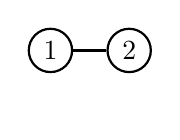
\begin{tikzpicture}[thick,
  every node/.style={circle,minimum width=.55cm, inner sep=1pt}
]
    \node[draw] (1) at (0,0) {1};
    \node[draw] (2) at (1,0) {2};
    \node[] () at (0,-.5) {};  // dummy node for padding at bottom
    \draw (1) -- (2);
\end{tikzpicture}
\qquad\quad
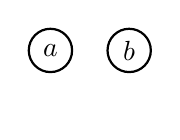
\begin{tikzpicture}[thick,
  every node/.style={circle,minimum width=.55cm, inner sep=1pt}
]
    \node[draw] (a) at (0,0) {$a$};
    \node[draw] (b) at (1,0) {$b$};
    \node[] () at (0,-.5) {};  // dummy node for padding at bottom
\end{tikzpicture}
\qquad\quad
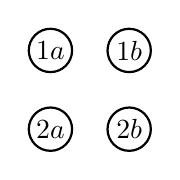
\begin{tikzpicture}[thick,
  every node/.style={draw,circle,minimum width=.55cm, inner sep=1pt}
]
    \node[draw] (1a) at (0,1) {$1a$};
    \node[draw] (1b) at (1,1) {$1b$};
    \node[draw] (2a) at (0,0) {$2a$};
    \node[draw] (2b) at (1,0) {$2b$};
\end{tikzpicture}
%%\begin{tikzpicture}[thick,
%%  every node/.style={draw,circle},
%%  class1node/.style={fill=myblue},
%%  class2node/.style={fill=mygreen},
%%  every fit/.style={ellipse,draw,inner sep=-2pt,text width=2cm}
%%]
%%        \graph [nodes={draw, circle, minimum width=.55cm, inner sep=1pt}, circular placement, radius=0.95cm,
%%                clockwise=2] {
%%                    1,2;
%%            1--2;
%%        };
%%\end{tikzpicture}
\qquad

\caption{Graphs $\graphG$ and $\graphH$ and their association graph $\graphA$.  \McSplit\
    gives an upper bound of 2 on the order of a maximum common induced subgraph
    of $\graphG$ and $\graphH$, whereas a clique algorithm computing
    a greedy colouring of $\graphA$ gives a tighter upper bound of 1.}
\label{fig:clique-better-bound}
\end{figure}

\Cref{fig:mcsplit-better-bound} shows an example in which \McSplit's bound
may be stronger than or equal to the clique bound depending on the order in
which the greedy colouring is carried out.  The input graphs are $K_2$ and
$K_3$.  Clearly, the \McSplit\ bound is 2.  A colouring of the association
graph has size either 2 (if we assign $1a$, $1b$, and $1c$
to one colour class, and $2a$, $2b$, and $2c$ to another) or 3 (if the
colour classes are $\{1a,2a\}$, $\{1b,2b\}$, and $\{1c,2c\}$).

\begin{figure}[htb]
\centering
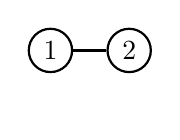
\begin{tikzpicture}[thick,
  every node/.style={circle,minimum width=.55cm, inner sep=1pt}
]
    \node[draw] (1) at (0,0) {1};
    \node[draw] (2) at (1,0) {2};
    \node[] () at (0,-.5) {};  // dummy node for padding at bottom
    \draw (1) -- (2);
\end{tikzpicture}
\qquad\quad
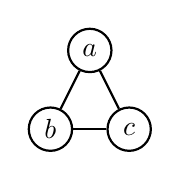
\begin{tikzpicture}[thick,
  every node/.style={circle,minimum width=.55cm, inner sep=1pt}
]
    \node[draw] (a) at (.5,1) {$a$};
    \node[draw] (b) at (0,0) {$b$};
    \node[draw] (c) at (1,0) {$c$};
    \draw (a) -- (b);
    \draw (a) -- (c);
    \draw (b) -- (c);
    %\node[] () at (0,-.5) {};  // dummy node for padding at bottom
\end{tikzpicture}
\qquad\quad
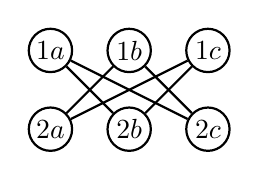
\begin{tikzpicture}[thick,
  every node/.style={draw,circle,minimum width=.55cm, inner sep=1pt}
]
    \node[draw] (1a) at (0,1) {$1a$};
    \node[draw] (1b) at (1,1) {$1b$};
    \node[draw] (1c) at (2,1) {$1c$};
    \node[draw] (2a) at (0,0) {$2a$};
    \node[draw] (2b) at (1,0) {$2b$};
    \node[draw] (2c) at (2,0) {$2c$};
    \draw (1a) -- (2b);
    \draw (1a) -- (2c);
    \draw (1b) -- (2a);
    \draw (1b) -- (2c);
    \draw (1c) -- (2a);
    \draw (1c) -- (2b);
\end{tikzpicture}
%%\begin{tikzpicture}[thick,
%%  every node/.style={draw,circle},
%%  class1node/.style={fill=myblue},
%%  class2node/.style={fill=mygreen},
%%  every fit/.style={ellipse,draw,inner sep=-2pt,text width=2cm}
%%]
%%        \graph [nodes={draw, circle, minimum width=.55cm, inner sep=1pt}, circular placement, radius=0.95cm,
%%                clockwise=2] {
%%                    1,2;
%%            1--2;
%%        };
%%\end{tikzpicture}
\qquad

\caption{Graphs $\graphG$ and $\graphH$ and their association graph $\graphA$.  \McSplit\
    gives an upper bound of 2 on the order of a maximum common induced subgraph
    of $\graphG$ and $\graphH$.  A greedy colouring of $\graphA$
    gives an upper bound of 2 or
    3, depending on the order in which vertices are coloured.}
\label{fig:mcsplit-better-bound}
\end{figure}

We now turn to the extreme case in which all vertex labels are distinct
in each of the two input graphs.  \Cref{fig:clique-bound-labelled} shows
two graphs, each with three distinctly labelled vertices; the labels
are represented by three different shapes.  The \McSplit\ upper bound is 3,
since there are three label classes, each containing one vertex from each graph.
A greedy colouring of the association graph gives a stronger bound, 2,
irrespective of the order in which the nodes are coloured, since
nodes $1a$ and $3c$ will be assigned to the same colour class.

\begin{figure}[htb]
\centering
\begin{tikzpicture}[thick,
  triangle/.style = {regular polygon, regular polygon sides=3, inner sep=0.2pt },
  square/.style = {regular polygon, regular polygon sides=4 },
  every node/.style={circle,minimum width=.55cm, inner sep=1pt}
]
    \node[draw,triangle] (1) at (.5,1) {1};
    \node[draw,square] (2) at (0,0) {2};
    \node[draw] (3) at (1,0) {3};
    \draw (1) -- (2);
    \draw (2) -- (3);
\end{tikzpicture}
\qquad\quad
\begin{tikzpicture}[thick,
  triangle/.style = {regular polygon, regular polygon sides=3, inner sep=0.7pt },
  square/.style = {regular polygon, regular polygon sides=4 },
  every node/.style={circle,minimum width=.55cm, inner sep=1pt}
]
    \node[draw,triangle] (a) at (.5,1) {$a$};
    \node[draw,square] (b) at (0,0) {$b$};
    \node[draw] (c) at (1,0) {$c$};
    \draw (a) -- (b);
    \draw (a) -- (c);
    \draw (b) -- (c);
    %\node[] () at (0,-.5) {};  // dummy node for padding at bottom
\end{tikzpicture}
\qquad\quad
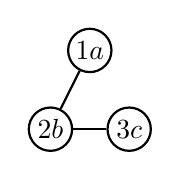
\begin{tikzpicture}[thick,
  every node/.style={draw,circle,minimum width=.55cm, inner sep=1pt}
]
    \node[draw] (1a) at (.5,1) {$1a$};
    \node[draw] (2b) at (0,0) {$2b$};
    \node[draw] (3c) at (1,0) {$3c$};
    \draw (1a) -- (2b);
    \draw (2b) -- (3c);
\end{tikzpicture}
%%\begin{tikzpicture}[thick,
%%  every node/.style={draw,circle},
%%  class1node/.style={fill=myblue},
%%  class2node/.style={fill=mygreen},
%%  every fit/.style={ellipse,draw,inner sep=-2pt,text width=2cm}
%%]
%%        \graph [nodes={draw, circle, minimum width=.55cm, inner sep=1pt}, circular placement, radius=0.95cm,
%%                clockwise=2] {
%%                    1,2;
%%            1--2;
%%        };
%%\end{tikzpicture}
\qquad

\caption{Graphs $\graphG$ and $\graphH$ and their association graph $\graphA$.
    Vertex labels are represented by shapes.  \McSplit\
    gives an upper bound of 3 on the order of a maximum common induced subgraph
    of $\graphG$ and $\graphH$.  A greedy colouring of $\graphA$
    gives an upper bound of 2.}
\label{fig:clique-bound-labelled}
\end{figure}

Clearly, this example generalises: if all of the vertices in each input
graph have distinct labels, then the clique bound is less than or equal to
the \McSplit\ bound.

We have established that the \McSplit\ and clique upper bounds are incomparable for unlabelled graphs,
and that the clique algorithm's bound is stronger than the \McSplit\ bound if there are very many vertex
labels. In fact, a bound calculated using greedy colouring can always be at least
as good as the \McSplit\ bound if we colour vertices in the right order; for example,
if we colour the vertices as described in the proof in \Cref{sec:mcsplit-proof}.

\paragraph{Experimental comparison of bounds}
Is the clique bound stronger in practice, even for unlabelled graphs?
We will see shortly that the answer is ``no''---at least if we use MCSa1 as the clique
algorithm.
To find the point at which the clique bound becomes preferable, I carried out a
small experiment on $G(n,p)$ random graphs, varying the size of the set of
vertex labels.

I generated 1800 pairs of random undirected, loopless graphs of order 20 without edge labels,
with densities ranging from $0.1$ to $0.9$
in steps of $0.1$.  For each integer value of a parameter $m$ (the maximum label) from 1 to 20, I generated
90 pairs of graphs with vertex labels assigned uniformly at random from the set $\{1,\dots,m\}$.  I used my
implementation of \McSplit\ and Prosser's implementation of the MCSa1 algorithm
\citep{DBLP:journals/algorithms/Prosser12} to find the \McSplit\ and clique bounds respectively
at the top of search (that is, on the first recursive call, before any vertex assignment decisions
have been made).

\Cref{figure:bound-ratio} plots the results of dividing the \McSplit\ upper bound by the
clique upper bound, with one point per instance.  The value of $m$ parameter is shown on the horizontal
axis; points towards the right of the plot have more distinct vertex labels.  Mean values
are shown as horizontal lines.  When $m=1$---that is,
when all vertices have the same label---the \McSplit\ bound is strictly tighter than the clique-algorithm
bound of all 90 of our instances.  On average, the \McSplit\ bound is tighter than the clique
bound for $m < 4$, and worse than the clique bound for $m > 5$.  Of the 900 instances with $m > 10$,
\McSplit\ had a tighter bound than the clique algorithm for only a single instance.

\begin{figure}[htb]
    \centering
    \includegraphics*[width=0.65\textwidth]{14-mcsplit-i-undirected/bound-experiments/plots/bounds-plot.pdf}
    \caption{As the number of vertex labels is increased, the clique algorithm's bound
    	becomes stronger than the \McSplit\ bound.
        The vertical axis shows the ratio of initial \McSplit\ upper bound
	to initial clique algorithm (MCSa1) upper bound for 1800 instances, with one dot per instance;
	for values less than 1, \McSplit's bound is better than that of the clique algorithm.
	The horizontal axis shows the maximum label $m$; each vertex label is a random integer 
	from the range $[1,m]$.}
    \label{figure:bound-ratio}
\end{figure}

To summarise, the upper bound of the clique encoding
dominates that of CP-FC and \McSplit\ where vertices are ``as labelled as possible'',
whereas neither bound dominates for unlabelled graphs.  Experimentally, we
see that the \McSplit\ bound is tighter than the clique bound for unlabelled
graphs, but the tightness of the clique bound steadily increases
relative to that of the \McSplit\ bound as the number of vertex
labels is increased.
This provides an explanation for the behaviour we saw in
\Cref{sec:mcsplit-experiments}, where \McSplit\ was the fastest solver
for unlabelled instances while the maximum clique solver was fastest for
instances with many distinct labels on vertices.

%A further advantage of our encoding is that it gives us efficient access to a
%better branching heuristic. The CP-FC algorithm uses smallest domain first,
%which in our algorithm corresponds to branching on a label class with smallest
%$|\setH|$. We instead branch on the label class with smallest $\max(|\setG|,|\setH|)$.
%This is empirically better, and accounts for much of the difference between
%the number of recursive calls made; branching on the smallest $|\setG| |\setH|$ gives
%very similar results. This can be viewed as exploiting both smallest domain first,
%and the dual viewpoint \citep{DBLP:conf/ecai/Geelen92} of smallest domain
%first, simultaneously, but we do not have the overheads of having to maintain
%and channel between the dual viewpoint that would be required when using a
%conventional domain store.

\section{Publications Using \McSplit}\label{sec:mcsplit-papers}

Since the \McSplit\ algorithm was published at IJCAI 2017, a number of papers, including
two that I co-authored, have further investigated the algorithm.
This section briefly surveys this work.

\subsection{Publications Co-Authored by the Present Author}

\citet{DBLP:conf/cpaior/ArchibaldDHMP019} introduce \emph{solution-biased search},
a technique using restarts and nogood learning that allows an algorithm to quickly explore diverse
parts of the search tree rather than explore it in
depth-first order (as a typical backtracking algorithm
such as the standard version of \McSplit\ does); this can often help the algorithm to find good
solutions quickly.  For the paper, I designed and implemented a version
of \McSplit\ using solution-biased search; this led to modestly improved run times on many instances.

In \citet{DBLP:conf/cp/GochtMMNPT20}, the present
author added proof logging \citep{DBLP:conf/ijcai/GochtMN20} to the C++ implementation of
\McSplit\ to create a \emph{certified} version of the solver.  This outputs a log of the
solver's reasoning steps using the cutting plane proof system
\citep{DBLP:journals/dam/CookCT87}, such that the log can be verified using a
simple and extensively tested checker program.  The proof logging and verification process
slows down the solver by around three orders of magnitude; therefore I did not use it for
the experiments in the current thesis chapter.  However, the program's logs were verified
for all 16,300 instances considered for the paper, providing evidence of the implementation's
correctness.

\subsection{Other Publications}

\citet{DBLP:conf/aaai/0001LJ020} introduce improved variable- and value-ordering
heuristics for \McSplit\ using reinforcement learning.
Specifically, when selecting a vertex in $\graphG$ or $\graphH$ to use for branching,
the algorithm prefers to use vertices that have resulted in a large decrease to the upper bound
in previous recursive calls.  This strategy enabled the new solver, \McSplit+RL,
to solve more instances within a time limit than \McSplit. Interestingly, a scatter
plot in the paper shows that each of \McSplit\ and \McSplit+RL is faster than
the other algorithm for many instances. This suggests that it could be useful
to include both algorithms in a portfolio solver.

\citet{DBLP:journals/computation/QuerMS20}
explore several enhancements of \McSplit,
including a massively parallel GPU implementation using CUDA, a recursion-free implementation,
and a parallel portfolio solver containing these along with the original \McSplit\
implementation.  The GPU implementation is shown to be promising although not competitive
with CPU implementations on the hardware used by the paper's authors; the portfolio solver,
however, is able to solve more instances within a given time limit than any of the
constituent solvers.

Finally, two theses --- the undergraduate thesis of Paulius Dilkas and
the Masters thesis of Jonathan Trummer --- make contributions
in both algorithm design and experimental work.

\citet{dilkas2018} performs a detailed experimental evaluation
of \McSplit\ and a clique algorithm for a range of labelling schemes, finding that \McSplit\
outperforms the clique encoding even for labelled graphs, if only a small number of labels are
used.  Dilkas uses machine learning to construct a portfolio solver that chooses intelligently
between \McSplit\ and the clique encoding according to easily computed characteristics of the
two input graphs such as density and standard deviation of degrees. The portfolio solver
outperforms each of its component algorithms, giving overall performance close to that of the virtual
best solver.  Finally, Dilkas constructs a hybrid algorithm, \textsc{Fusion}, that switches
from \McSplit\ to the clique encoding at a specified depth of recursion.

\cite{trummer2021} presents several innovations for maximum common induced subgraph algorithms,
including improved reinforcement learning for \McSplit\ based on
\citet{DBLP:conf/aaai/0001LJ020}, and a version of \McSplit\ with symmetry breaking.

\subsection{An Application to a Question in Probability Theory}

Chatterjee and Diaconis \cite{chatterjee2021isomorphisms} consider taking two
independent random $G(N, 1/2)$ graphs $G$ and $H$, and finding the order of their maximum
common induced subgraph.  They prove that as $N\to\infty$, the maximum common
subgraph of $G$ and $H$ will, with probability tending to 1, be in a range
consisting of either one integer or two consecutive integers.  This range
is given by $\{\lfloor x_N - \varepsilon_N\rfloor, \lfloor x_N + \varepsilon_N\rfloor\}$,
where $x_N = 4 \log_2 N - 2 \log_2\log_2 N - 2 \log_2(4/e) + 1$
and $\varepsilon_N = (4 \log_2 N)^{-1/2}$.  It is interesting to examine whether
this precise prediction of the order of a maximum common induced subgraph
comes close to holding, even for small values of $N$.

\Cref{figure:mcis-order-bands}
shows data provided by the present author to Chatterjee and Diaconis; a subset
of this data is presented in their paper.  The broad blue bands give the
range of predicted MCIS orders for a given $N$; each band is either a single
integer or a range of two consecutive integers.  The orange points show the mean
MCIS orders for randomly generated pairs of graphs, and the bands show the
range of MCIS orders observed.  For $N \leq 32$, 100 pairs of graphs were
generated.  Due to the difficulty of solving larger instances, one pair
of graphs was generated for each $N$ in the range $32 < N \leq 45$.  For values
of $N$ above 27, the theorem of Chatterjee and Diaconis is a good predictor
of the MCIS size, differing by at most 1 from the values observed in our
generated data.

\begin{figure}[htb]
    \centering
    \includegraphics*[width=0.7\textwidth]{14-mcsplit-i-undirected/data-for-diaconis-and-chatterjee/plot}
    \caption{For each $N$, the blue bands give the range of predicted maximum
    common induced subgraph orders given by the asymptotic formula by
    Chatterjee and Diaconis \cite{chatterjee2021isomorphisms}.  For $N \leq 32$,
    100 instances were generated; the orange bands give the range of MCIS orders
    observed, and the orange points give the means.  For $32 < N \leq 45$,
    a single instance was generated; the MCIS order is shown as a single point.}
    \label{figure:mcis-order-bands}
\end{figure}

\section{Conclusion}
\label{sec:mcsplit-conclusion}

This chapter has introduced the \McSplit\ algorithm for maximum common induced subgraph
problems, which is more than an order of magnitude faster than the
previous state of the art for unlabelled, undirected instances. We have
seen how the algorithm can be extended for graphs with labels on edges, labels
on vertices, loops, directed edges and the requirement that the resultant graph
be connected.  We have also explored the large effect that sorting graphs
by degree can have on run times, and examined the relationship between the upper bounds
calculated by \McSplit\ and by clique algorithms.

%It would be interesting in the future to see whether the data structures and
%partitioning algorithms of \McSplit\ have applicability beyond subgraph
%problems---the author suspects that some other problems may have a similar
%branching structure which would also benefit from a partitioning domain store
%representation. Most obviously, we could solve the induced subgraph isomorphism
%problem in the same way (and with nearly no changes to the code), and our
%connected variant shows that certain side constraints can also be handled.
%However, we cannot solve non-induced subgraph isomorphism this way, nor can we
%handle certain richer labelling schemes such as those used in temporal subgraph
%isomorphism \citep{DBLP:conf/asunam/RedmondC13}.

% \section{Commented out recycle bin}
% 
% FROM THE INTRO
% 
% To determine the similarity or difference between two graphs, we must first
% find what they have in common
% \citep{DBLP:journals/prl/Bunke97,DBLP:journals/prl/FernandezV01,KriegeThesis}.
% The \emph{maximum common subgraph} family of problems involves finding a large
% graph which is isomorphic to subgraphs of two given graphs simultaneously.
% Because graphs are widely used to model real-world phenomena, maximum common
% subgraph problems have arisen in molecular science (where graphs often represent
% molecules)
% \citep{DBLP:journals/jcamd/RaymondW02a,Ehrlich:2011,DAM2014,Grindley1993707},
% and also in other domains including malware detection
% \citep{DBLP:journals/compsec/ParkRS13}, source code analysis
% \cite{DBLP:journals/tkde/DjokoCH97}, and computer vision
% \cite{DBLP:journals/jair/CookH94}.
% 
% Maximum common subgraph problems are \NP-hard, and remain challenging
% computationally. Recent practical progress has been made by using constraint
% programming \citep{DBLP:conf/mco/VismaraV08,DBLP:conf/cp/NdiayeS11,DBLP:conf/cp/McCreeshNPS16} and
% mathematical programming \citep{DBLP:journals/dam/BahienseMPS12}, by reducing
% to the maximum clique problem \citep{LeviG,DBLP:conf/cp/McCreeshNPS16}, and by
% adapting subgraph isomorphism algorithms \citep{UpcomingAAAIPaper}. Some
% special cases also have practical polynomial time algorithms
% \citep{DBLP:conf/mfcs/DroschinskyKM16,DBLP:conf/sofsem/DroschinskyKM17}.
% 
% This chapter considers the \emph{maximum common induced subgraph} problem, in
% which the objective is to find a graph with as many vertices as possible which
% is an induced subgraph of each of two input graphs.  (The \emph{maximum common
% partial subgraph} problem instead asks for a common non-induced subgraph with
% as many \emph{edges} as possible \citep{DBLP:conf/cp/NdiayeS11}; we discuss
% only the induced variant in this chapter.) We introduce
% a new branch and bound algorithm which exploits special properties of the
% problem to allow a much faster exploration of the search space, whilst
% retaining the filtering and bounding benefits of the constraint programming
% approach. We describe the algorithm for the basic maximum common subgraph
% problem, and discuss how it may be adapted to handle vertex labels, edge
% labels, and the requirement that the found subgraph be connected. We then
% present an empirical study of the algorithm, demonstrating that it improves the
% state of the art by more than an order of magnitude on the unlabelled variant
% of the problem, and showing that it can handle much larger instances than
% earlier constraint programming or clique approaches due to lower memory usage.
% 
% FROM START OF PROOF SECTION (ROUGHLY DUPLICATES BACKGROUND CHAPTER)
%
%\Cref{fig:association-graph} shows the association graph of graphs $\graphG$ and $\graphH$
%from \cref{fig:alg1}, which has 30 vertices and 150 edges.  A 4-clique corresponding to
%a maximum common subgraph of $\graphG$ and $\graphH$ is shown.
%
%\begin{figure}[htb]
%\centering
%    \begin{tikzpicture}
%        \foreach \v [count=\i] in {1,2,3,4,5} {
%            \foreach \w [count=\j] in {a,b,c,d,e,f} {
%                \node[draw,circle,minimum width=.58cm,inner sep=1pt] (\v\w) at (180 - \i*72 - \j*11:4.1) {$\v\w$};
%            }
%        }
%        \draw[color=gray, line width=.3] (1a) -- (2d);
\draw[color=gray, line width=.3] (1a) -- (3f);
\draw[color=gray, line width=.3] (1a) -- (4b);
\draw[color=gray, line width=.3] (1a) -- (4c);
\draw[color=gray, line width=.3] (1a) -- (4e);
\draw[color=gray, line width=.3] (1a) -- (5c);
\draw[color=gray, line width=.3] (1a) -- (5e);
\draw[color=gray, line width=.3] (1b) -- (2c);
\draw[color=gray, line width=.3] (1b) -- (2e);
\draw[color=gray, line width=.3] (1b) -- (3c);
\draw[color=gray, line width=.3] (1b) -- (3e);
\draw[color=gray, line width=.3] (1b) -- (4a);
\draw[color=gray, line width=.3] (1b) -- (4d);
\draw[color=gray, line width=.3] (1b) -- (4f);
\draw[color=gray, line width=.3] (1b) -- (5a);
\draw[color=gray, line width=.3] (1b) -- (5d);
\draw[color=gray, line width=.3] (1b) -- (5f);
\draw[color=gray, line width=.3] (1c) -- (2b);
\draw[color=gray, line width=.3] (1c) -- (3b);
\draw[color=gray, line width=.3] (1c) -- (4a);
\draw[color=gray, line width=.3] (1c) -- (4d);
\draw[color=gray, line width=.3] (1c) -- (4e);
\draw[color=gray, line width=.3] (1c) -- (4f);
\draw[color=gray, line width=.3] (1c) -- (5a);
\draw[color=gray, line width=.3] (1c) -- (5d);
\draw[color=gray, line width=.3] (1c) -- (5e);
\draw[color=gray, line width=.3] (1c) -- (5f);
\draw[color=gray, line width=.3] (1d) -- (2a);
\draw[color=gray, line width=.3] (1d) -- (2e);
\draw[color=gray, line width=.3] (1d) -- (3a);
\draw[color=gray, line width=.3] (1d) -- (3e);
\draw[color=gray, line width=.3] (1d) -- (4b);
\draw[color=gray, line width=.3] (1d) -- (4c);
\draw[color=gray, line width=.3] (1d) -- (4f);
\draw[color=gray, line width=.3] (1d) -- (5b);
\draw[color=gray, line width=.3] (1d) -- (5c);
\draw[color=gray, line width=.3] (1d) -- (5f);
\draw[color=gray, line width=.3] (1e) -- (2b);
\draw[color=gray, line width=.3] (1e) -- (2d);
\draw[color=gray, line width=.3] (1e) -- (3b);
\draw[color=gray, line width=.3] (1e) -- (3d);
\draw[color=gray, line width=.3] (1e) -- (4a);
\draw[color=gray, line width=.3] (1e) -- (4c);
\draw[color=gray, line width=.3] (1e) -- (4f);
\draw[color=gray, line width=.3] (1e) -- (5a);
\draw[color=gray, line width=.3] (1e) -- (5c);
\draw[color=gray, line width=.3] (1e) -- (5f);
\draw[color=gray, line width=.3] (1f) -- (2a);
\draw[color=gray, line width=.3] (1f) -- (3a);
\draw[color=gray, line width=.3] (1f) -- (4b);
\draw[color=gray, line width=.3] (1f) -- (4c);
\draw[color=gray, line width=.3] (1f) -- (4d);
\draw[color=gray, line width=.3] (1f) -- (4e);
\draw[color=gray, line width=.3] (1f) -- (5b);
\draw[color=gray, line width=.3] (1f) -- (5c);
\draw[color=gray, line width=.3] (1f) -- (5d);
\draw[color=gray, line width=.3] (1f) -- (5e);
\draw[color=gray, line width=.3] (2a) -- (3b);
\draw[color=gray, line width=.3] (2a) -- (3c);
\draw[color=gray, line width=.3] (2a) -- (3e);
\draw[color=gray, line width=.3] (2a) -- (4d);
\draw[color=gray, line width=.3] (2a) -- (4f);
\draw[color=gray, line width=.3] (2a) -- (5b);
\draw[color=gray, line width=.3] (2a) -- (5c);
\draw[color=gray, line width=.3] (2a) -- (5e);
\draw[color=gray, line width=.3] (2b) -- (3a);
\draw[color=gray, line width=.3] (2b) -- (3d);
\draw[color=gray, line width=.3] (2b) -- (3f);
\draw[color=gray, line width=.3] (2b) -- (4c);
\draw[color=gray, line width=.3] (2b) -- (4e);
\draw[color=gray, line width=.3] (2b) -- (5a);
\draw[color=gray, line width=.3] (2b) -- (5d);
\draw[color=gray, line width=.3] (2b) -- (5f);
\draw[color=gray, line width=.3] (2c) -- (3a);
\draw[color=gray, line width=.3] (2c) -- (3d);
\draw[color=gray, line width=.3] (2c) -- (3e);
\draw[color=gray, line width=.3] (2c) -- (3f);
\draw[color=gray, line width=.3] (2c) -- (4b);
\draw[color=gray, line width=.3] (2c) -- (5a);
\draw[color=gray, line width=.3] (2c) -- (5d);
\draw[color=gray, line width=.3] (2c) -- (5e);
\draw[color=gray, line width=.3] (2c) -- (5f);
\draw[color=gray, line width=.3] (2d) -- (3b);
\draw[color=gray, line width=.3] (2d) -- (3c);
\draw[color=gray, line width=.3] (2d) -- (3f);
\draw[color=gray, line width=.3] (2d) -- (4a);
\draw[color=gray, line width=.3] (2d) -- (4e);
\draw[color=gray, line width=.3] (2d) -- (5b);
\draw[color=gray, line width=.3] (2d) -- (5c);
\draw[color=gray, line width=.3] (2d) -- (5f);
\draw[color=gray, line width=.3] (2e) -- (3a);
\draw[color=gray, line width=.3] (2e) -- (3c);
\draw[color=gray, line width=.3] (2e) -- (3f);
\draw[color=gray, line width=.3] (2e) -- (4b);
\draw[color=gray, line width=.3] (2e) -- (4d);
\draw[color=gray, line width=.3] (2e) -- (5a);
\draw[color=gray, line width=.3] (2e) -- (5c);
\draw[color=gray, line width=.3] (2e) -- (5f);
\draw[color=gray, line width=.3] (2f) -- (3b);
\draw[color=gray, line width=.3] (2f) -- (3c);
\draw[color=gray, line width=.3] (2f) -- (3e);
\draw[color=gray, line width=.3] (2f) -- (4a);
\draw[color=gray, line width=.3] (2f) -- (5c);
\draw[color=gray, line width=.3] (2f) -- (5d);
\draw[color=gray, line width=.3] (2f) -- (5e);
\draw[color=gray, line width=.3] (3a) -- (4d);
\draw[color=gray, line width=.3] (3a) -- (4f);
\draw[color=gray, line width=.3] (3a) -- (5b);
\draw[color=gray, line width=.3] (3a) -- (5c);
\draw[color=gray, line width=.3] (3a) -- (5e);
\draw[color=gray, line width=.3] (3b) -- (4c);
\draw[color=gray, line width=.3] (3b) -- (4e);
\draw[color=gray, line width=.3] (3b) -- (5a);
\draw[color=gray, line width=.3] (3b) -- (5d);
\draw[color=gray, line width=.3] (3b) -- (5f);
\draw[color=gray, line width=.3] (3c) -- (4b);
\draw[color=gray, line width=.3] (3c) -- (5a);
\draw[color=gray, line width=.3] (3c) -- (5d);
\draw[color=gray, line width=.3] (3c) -- (5e);
\draw[color=gray, line width=.3] (3c) -- (5f);
\draw[color=gray, line width=.3] (3d) -- (4a);
\draw[color=gray, line width=.3] (3d) -- (4e);
\draw[color=gray, line width=.3] (3d) -- (5c);
\draw[color=gray, line width=.3] (3d) -- (5f);
\draw[color=gray, line width=.3] (3e) -- (4b);
\draw[color=gray, line width=.3] (3e) -- (4d);
\draw[color=gray, line width=.3] (3e) -- (5a);
\draw[color=gray, line width=.3] (3e) -- (5c);
\draw[color=gray, line width=.3] (3e) -- (5f);
\draw[color=gray, line width=.3] (3f) -- (4a);
\draw[color=gray, line width=.3] (3f) -- (5b);
\draw[color=gray, line width=.3] (3f) -- (5c);
\draw[color=gray, line width=.3] (3f) -- (5d);
\draw[color=gray, line width=.3] (3f) -- (5e);
\draw[color=gray, line width=.3] (4a) -- (5d);
\draw[color=gray, line width=.3] (4a) -- (5f);
\draw[color=gray, line width=.3] (4b) -- (5c);
\draw[color=gray, line width=.3] (4b) -- (5e);
\draw[color=gray, line width=.3] (4c) -- (5b);
\draw[color=gray, line width=.3] (4d) -- (5a);
\draw[color=gray, line width=.3] (4d) -- (5e);
\draw[color=gray, line width=.3] (4e) -- (5b);
\draw[color=gray, line width=.3] (4e) -- (5d);
\draw[color=gray, line width=.3] (4f) -- (5a);
\draw[ultra thick] (1a) -- (2f);
\draw[ultra thick] (1a) -- (3d);
\draw[ultra thick] (1a) -- (5b);
\draw[ultra thick] (2f) -- (3d);
\draw[ultra thick] (2f) -- (5b);
\draw[ultra thick] (3d) -- (5b);

%    \end{tikzpicture}   
%\caption{The association graph of graphs $\graphG$ and $\graphH$ from \cref{fig:alg1}.  The dark edges
%    show a 4-clique in
%    the association graph. This corresponds to a common subgraph with 4 vertices: the subgraph of $\graphG$ induced by
%    $\{1,2,3,5\}$ which is isomorphic to the subgraph of $\graphH$ induced by $\{a,f,d,b\}$.}
%\label{fig:association-graph}
%\end{figure}

% SIP INSTANCES
%
%\begin{figure}[htb]
%    \centering
%    \includegraphics*[width=0.75\textwidth]{14-mcsplit-i-undirected/img/gen-graph-sip-cumulative.pdf}
%    \caption{Cumulative numbers of instances solved over time for the maximum
%    common connected subgraph problem on the large subgraph isomorphism benchmark
%    suite.} \label{figure:sip-cumulative}
%\end{figure}
%
%\paragraph{Large subgraph isomorphism instances} We also ran the algorithms on
%a set of 5,725 larger instances used in recent studies of subgraph
%isomorphism~\citep{DBLP:conf/lion/KotthoffMS16} and maximum common
%subgraph~\citep{UpcomingAAAIPaper}.  This benchmark set includes real-world
%graphs and graphs generated using random models.  Pattern graphs range from 4
%vertices to 900 with a median of 80; target graphs range from 10 vertices to
%6,671 with a median of 561. Cumulative runtimes on these instances are shown in
%\cref{figure:sip-cumulative}.  This is a challenging set of instances, and more
%than half of the instances cannot be solved within a timeout of 1,000 seconds by
%any solver. Furthermore, the CP-FC algorithm and the clique encoding run out of
%memory on many of the instances (these are treated as timeouts, following
%\citet{UpcomingAAAIPaper}).
%
%    \par\bigskip
%    \subfigure[][Subgraph isomorphism instances]{\label{figure:prettyheatmaps3}
%       \includegraphics*[width=.5\textwidth]{14-mcsplit-i-undirected/img/gen-graph-sip-james-versus-kdown-nodes-scatter.pdf}
%    }
%What about our relationship to the $k{\downarrow}$ of
%\citet{UpcomingAAAIPaper}?  \Cref{figure:prettyheatmaps3} plots the number of
%recursive calls made by $k{\downarrow}$ and \McSplit{$\downarrow$} on each of the subgraph
%isomorphism instances. Although \McSplit{$\downarrow$} is the faster of the two algorithms overall, it
%explores more search nodes than $k{\downarrow}$ for most instances (even taking
%into account that $k{\downarrow}$ uses a unit propagation loop, and so measures
%the search tree slightly differently). This is the classic tradeoff between
%speed and cleverness. A hybrid algorithm could be beneficial here: it could use
%$k{\downarrow}$ initially, switching to \McSplit{$\downarrow$} when the extra filtering is
%ineffective, and finally switching to a clique encoding when fewer than some
%threshold number of vertices remain to be selected. This might deliver the
%benefits of the clique encoding for labelled graphs, while avoiding the high
%memory cost and colouring time of encoding the full instance.
% 
% The basic \McSplit\ is beaten by $k{\downarrow}$ 
% \citet{UpcomingAAAIPaper} on this dataset. However, as
% \cref{figure:sip-cumulative} shows, \McSplitDown\ is the overall strongest
% algorithm on these instances for every choice of timeout.
% In many cases the maximum common subgraph covers nearly all of the smaller graph;
% thus, it is unsurprising that \kDown\ and \McSplitDown\ outperform the branch-and-bound
% \McSplit\ on this set of instances.
% %%% * The commented lines below are incorrect. *
% %%%(By contrast, the optimal solutions for the instances in
% %%%\cref{figure:mcs-cumulative-plain-not-connected},
% %%%\cref{figure:mcs-cumulative-labelled-not-connected}
% %%%and
% %%%\cref{figure:mcs-cumulative-connected} typically cover a smaller proportion of the
% %%%input graphs, and \McSplit{$\downarrow$} is often more than a magnitude slower than
% %%%the plain \McSplit\ algorithm for these instances; the \McSplit{$\downarrow$} results
% %%%are not shown for these instances.)
% 

% MAIN EXPERIMENTS
% TODO: re-run experiments using \McSplitDown\ and don't use \McSplit-D.
% Why does \McSplitDown\ seldom take more than twice as long as \McSplit,
% and why is it often much faster?  To answer this question, we implemented
% a slightly simplified version of \McSplitDown\ that (like \McSplitDown)
% solves the maximum
% common subgraph problem by a sequence of decision problems, and
% (unlike \McSplitDown) does not share an incumbent between calls to the decision-problem solver.
% We call this variant \McSplit-D.  We ran this on a subset of
% the plain MCS instances with a time limit of 100 seconds, and measured the
% time taken for each decision-problem solution.
% 
% Clearly, all of the decision problems are unsatisfiable except the final one,
% in which the target graph order equals the order of a maximum common subgraph.
% \Cref{figure:decision-scatter-last-two-all-others} plots the time required
% to solve the last two subproblems --- one unsatisfiable, one satisfiable ---
% against the time taken to solve all other
% subproblems.  (TODO: say if any instances had no unsat decision problems.)
% Without exception, more than half of the total time to solve
% each instance was spent on the last two decision problems.
% 
% It can be proven that each of these two final decision problems has a search tree that is no larger
% than the search tree of the branch-and-bound \McSplit.  For the final (satisfiable)
% instance, the search tree explored by \McSplit-D is equivalent
% to the search tree that would be explored by \McSplit\ if we initially set the incumbent
% to be one vertex smaller than the optimal solution, then stopped searching upon finding
% an optimal solution.  For the penultimate (unsatisfiable) instance, the search
% tree explored by \McSplit-D is equivalent to the search tree that would be explored by
% \McSplit\ if we initially set the incumbent equal to an optimal solution.
% 
% To summarise our discussion so far: each of the final two decision problems solved by \McSplit-D can
% be shown to require a search tree no larger than the full \McSplit\ search tree; furthermore,
% we have seen empirically that these two decision problems together take the majority of
% the run time of \McSplit-D.  These facts together explain why \McSplit\ is never much faster
% than \McSplit-D.
%
%Although it does not affect the foregoing argument,
%\Cref{figure:decision-scatter-last-two} compares, for completeness, the
%run times of the last two decision problems for each instance.  In most cases, the final
%unsatisfiable instance takes longer to solve than the satisfiable instance.
%
%\begin{figure}[h!]
%    \centering
%    \subfigure[][Last two decision problems vs all other decision problems] {
%        \centering
%        \includegraphics*[width=0.4\textwidth]{14-mcsplit-i-undirected/modified-mcsplit-experiment/plots/plots/decision-problems-last-two-all-others}
%        \label{figure:decision-scatter-last-two-all-others}
%    }
%    \subfigure[][Last two decision problems] {
%        \centering
%        \includegraphics*[width=0.4\textwidth]{14-mcsplit-i-undirected/modified-mcsplit-experiment/plots/plots/decision-problems-last-two}
%        \label{figure:decision-scatter-last-two}
%    }
%    \caption{Run times in ms of decision subproblems using the solver \McSplit-D, which solves
%        the maximum common subgraph problem by solving a sequence of decision problems.  Instances
%        that were not solved to optimality within the time limit are not shown.}\label{figure:decision-problem-time-scatters}
%\end{figure}

